%!TeX root = 3-fastsim.tex
\documentclass[main]{subfiles}

\begin{document}

\chapter{Adsorption Energies Sampling}
\vspace*{-1\baselineskip}

\section{Voronoi sampling}

\subsection{Theoretical considerations}

In mathematics, a tessellation of a given space corresponds to a partition into non overlapping sub-spaces. In the Voronoi tessellation, named after Georgy Feodosevich Voronoy, a set of points (seeds) are associated to a tessellation of regions (Voronoi cells) so that each seed has a cell whose points are closer to this seed than any other seeds.\cite{Rycroft_2009} Applied in materials science, the Voronoi cells associated to each atom of the framework can be used to determine key geometrical descriptors (void volume, accessible surface area, pore sizes). At the vertices of each cell, there are Voronoi nodes that was used in the Voronoi energy calculation presented by Simon et al.\cite{Simon2015}

\subsubsection{Equal radii}

In a tridimensionnal space, let us consider the positions ${(\vect{x}_k)}_{k\in\{1,\ldots,n\}}$ of the $n$ points in a box $B$ that could be periodically propagated in the whole space. For every $k\in\{1,\ldots,n\}$, we can then define a subspace $S_{k}$ (also called Voronoi cell) around the atom $k$ so that any point $\vect{x}$ inside this subspace is closer to the position $\vect{x}_k$ than to any other points $\vect{x}_l$ ($l\neq k$). 

\begin{equation}\label{eq:voronoi_partition}
  S_{k} = \left\{\vect{x} \in B\ \ |\ \ \forall\ l\neq k,\ \lVert \vect{x}-\vect{x}_k \rVert \leq \lVert \vect{x}-\vect{x}_l \rVert \right\}
\end{equation}

The set of all these 3D polyhedronal subspaces $S_{k}$ is then called the Voronoi partition of the space $B$. The edges and vertices of these polyhedra can then give valuable informations of the void space between the adjacent Voronoi cells associated to them. We can quickly use them to determine the accessible and inaccessible points of the void space. For instance, a vertex $\vect{v}$ of $p$ subspaces $\left\{V_{i_1},\ldots,V_{i_p}\right\}$ is the closest point to the atomic positions $\vect{x}_{i_1},\ldots,\vect{x}_{i_p}$ --- this can simply be proved by combining the different conditions of equation~\ref{eq:voronoi_partition}. The same assessment can be done for any point on an edge adjacent to some subspaces, it will be closer to the atoms associated with these subspaces than to any other atoms.

\begin{figure}
    \centering
    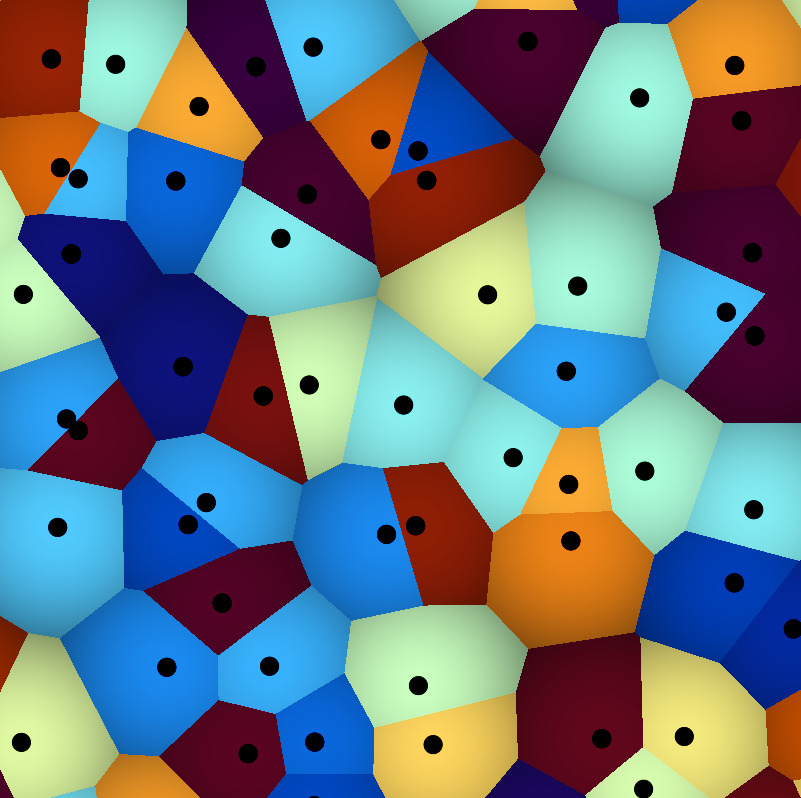
\includegraphics[width=0.4\textwidth]{figures/3-fastsim/voronoi.jpg}
    \caption{2D Voronoi. \url{https://www.shadertoy.com/view/MslGD8}}\label{fgr:voronoi_equal}
  \end{figure}

\subsubsection{Unequal radii}

The last definition of the Voronoi decomposition works only for equal-sized atoms because the closest region to an atom is also the closest to its center of mass, which does not apply to the complex atomic structures of nanoporous frameworks. To model the atomic radii $\vect{r}_1,\ldots,\vect{r}_n$ of the points $\vect{x}_1,\ldots,\vect{x}_n$ in the same box $B$, we can implement a so-called Apollonian Voronoi diagram.\cite{voronoi_apollonian} For every $k\in\{1,\ldots,n\}$, the new subspaces $A_{k}$ are defined as follows:

\begin{equation}\label{eq:r_voronoi_apollonian}
  A_{k} = \left\{\vect{x} \in B\ \ |\ \ \forall\ l\neq k,\ \lVert \vect{x}-\vect{x}_k \rVert - r_k \leq \lVert \vect{x}-\vect{x}_l \rVert - r_l \right\}
\end{equation}

This new definition of the Voronoi diagram has been built on the intuitive property that stipulates that the subspace is the set of points closest to the surface of the sphere around the associated atom. It deals therefore with an unequal distribution of atomic radii, because it is now dependent on the radii. However, as we can see on the Figure~\ref{fgr:voronoi_unequal}, this first implementation has a very convenient definition but the edges of the subspaces are curved, which makes it harder to use computationally. 

\begin{figure}
    \centering
    
\includegraphics[width=0.4\textwidth]{figures/3-fastsim/voronoi_apollonian.jpg}
    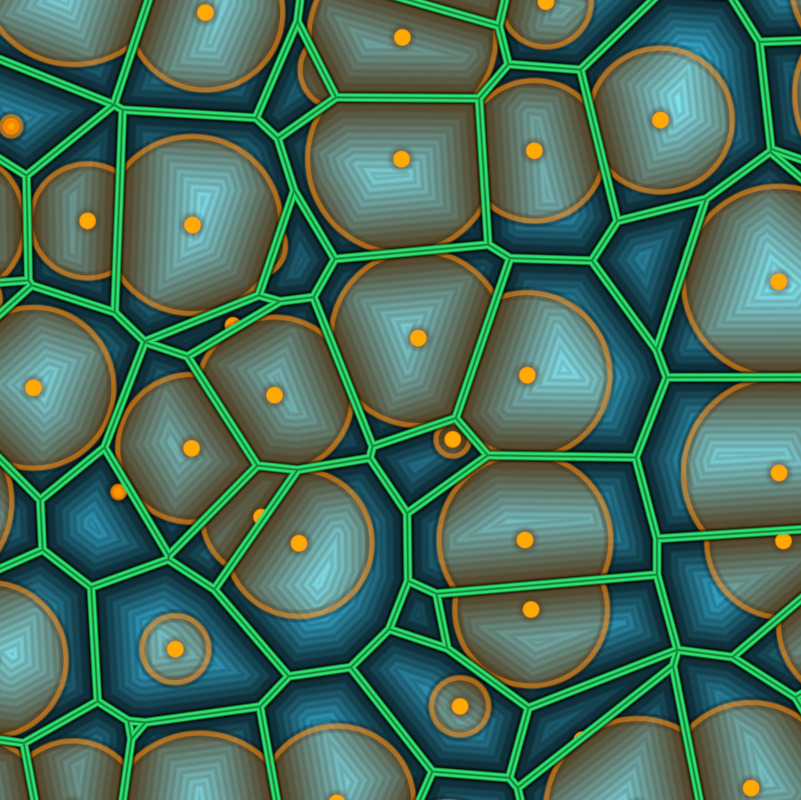
\includegraphics[width=0.4\textwidth]{figures/3-fastsim/voronoi_radical.jpg}
    \caption{2D Apollonian Voronoi decomposition. \url{https://www.shadertoy.com/view/4sd3D7} / Radical Voronoi decomposition. \url{https://www.shadertoy.com/view/4tV3z3}}\label{fgr:voronoi_unequal}
  \end{figure}

For this reason a less intuitive implementation is more commonly used instead, which is called the radical Voronoi tesselation or power diagram or Laguerre-Voronoi diagram.\cite{aurenhammer_1987} As we can see on the Figure~\ref{fgr:voronoi_unequal}, the subspaces obtained using this method are now convex polygons with straight edges instead of curved ones. The condition is way less intuitive because it the condition does not rely on a simple definition. The subspaces $V_k$ are now defined by the following condition:

\begin{equation}\label{eq:r_voronoi_radical}
    V_{k} = \left\{\vect{x} \in B\ \ |\ \ \forall\ l\neq k,\ \lVert \vect{x}-\vect{x}_k \rVert^2 - r_k^2 \leq \lVert \vect{x}-\vect{x}_l \rVert^2 - r_l^2 \right\}
  \end{equation}

In addition to the polyhedral form of the Voronoi cells, this new implementation presents interesting properties for porosity calculations in a framework of unequal spheres like in MOFs of zeolites.\cite{voronoi_radical} First, the boundary between two overlapping spheres correspond simply to the intersection place between the spheres. Then, the boundary between non-overlapping spheres is always in the void space between the spheres. This can be simply proven by taking a point $\vect{x}$ in $V_{k}$ and outside the sphere, we have $\lVert \vect{x}-\vect{x}_k \rVert \geq r_k$, which implies $\forall\ l\neq k$, $\lVert \vect{x}-\vect{x}_k \rVert \geq r_k$. The point $\vect{x}$ is therefore also not overlapping with any other atom, which means it is in the void space of the framework. 

If we now consider a point $\vect{v}$ on a boundary between $p$ Voronoi cells $\left\{V_{i_1},\ldots,V_{i_p}\right\}$, this point would verify all the conditions $\lVert \vect{x}-\vect{x}_{i_1} \rVert^2 - r_{i_1}^2 = \cdots = \lVert \vect{x}-\vect{x}_{i_p} \rVert^2 - r_{i_p}^2 = C$. We can know their minimum distance to the center of mass of every nearby atoms to test for possible overlappings. More specifically, in the Zeo++ software,\cite{Zeo++} the Voronoi diagram is characterized by storing the minimum distance to the closest atoms and the index of the atoms for every vertices and edges (for edges that connect two different periodic images a periodic displacement vector is also stored). This information can be used to speed up the void fraction calculation, by skipping the volume calculations in the non-adsorbable Voronoi cells. It is also a fast way of determining the accessible and non-accessible surface areas and volumes.\cite{Zeo++} Note that if the probe has a radius $r\e{probe}$, then the sphere radii considered are $r_k = r\e{atom}+r\e{probe}$.

\subsection{Implementation in a Screening}

The use of the Voronoi decomposition of the pore space of materials for their geometric characterization has been widely employed in computational studies in the last decade,\cite{Willems_2012} in particular since it was made easily available as part of the Zeo++ software package.\cite{Pinheiro2013} Its use was extended recently to implement a novel sampling scheme, in a study proposing the ML-assisted screening of nanoporous materials for xenon/krypton separation. In this article, Simon et al.\cite{Simon_2015} relied on a Voronoi tessellation of the nanoporous materials and assigned the potential adsorption sites (i.e., the sampling points) at the nodes of this decomposition. The Voronoi tessellation identifies the vertices of polyhedra that correspond to the closest regions of each atom of the structure. These vertices (or \emph{Voronoi nodes}) are the points equidistant to at least four atoms of the structure, and they can be associated with adsorption sites since they are positioned near the center of the pores. 

The definition of accessibility defined by the Zeo++ software was used in a screening to find the best materials for Xe/Kr separation.\ref{Simon_2015} The interaction energies of xenon were calculated only on the accessible nodes as schemed on the Figure~\ref{fgr:simon_voro}. The average of the energies at the accessible Voronoi nodes gives an approximation of the adsorption enthalpy. However, this sampling assumes that the nodes are close to the real, most favorable, adsorption sites. Or to put it differently, the adsorption sites need to be at the center of the pores, which is only true for structures with pore sizes close to adsorbate size. This newly defined adsorption energy descriptor was found to be one of the most influencial descriptor for the ML model developed to predict the ambient-pressure selectivity. 

\begin{figure}
  \centering
  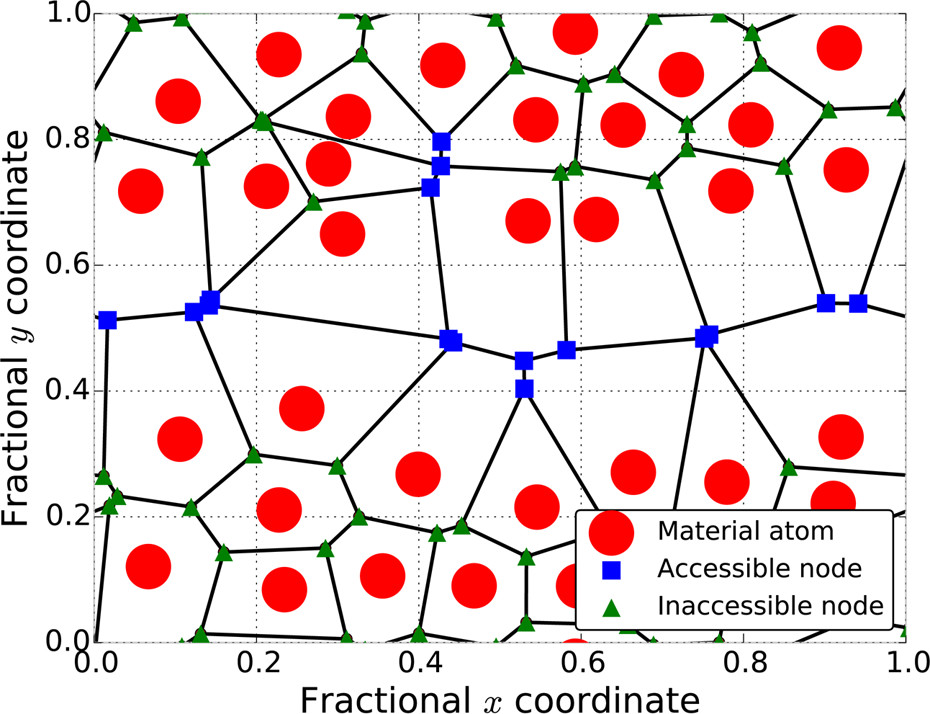
\includegraphics[width=0.6\textwidth]{figures/3-fastsim/Simon_voronoi.jpeg}
  \caption{Voronoi network model of void space (2D caricature). The unit cell of a toy material is shown. Red circles represent atoms of the material; accessible and inaccessible Voronoi nodes are blue squares and green triangles, respectively. The black lines are the edges in the periodic Voronoi graph that model the void space. Taken from Ref.~\cite{Simon_2015}}\label{fgr:simon_voro}
\end{figure}

Starting from the initial idea of Voronoi sampling, we want to question the relevance of using a direct average of the interaction energies instead of a Boltzmann averaging in describing the adsorption enethalpy. To better understand the strengths and weaknesses of this methodology, we compared different ways of approximating adsorption enthalpies using the Voronoi sampling with more accurate infinite dilution and ambient-pressure xenon adsorption enthalpies using Widom insertions and GCMC for a 20:80 xe/Kr mixture at \SI{1}{\atm} and \SI{298}{\kelvin}.

\subsection{Comparative study of the Voronoi sampling}

We introduced in the previous chapter, the definition of the xenon adsorption enthalpy at infinite dilution (Widom insertion section 2.1.3) and at ambient pressure (GCMC sections 2.1.2 and 2.1.4). These methods can be considered accurate methods to calculate the adsorption enthalpy which has been prove to be strongly correlated to the logarithm of the selectivity in the our previous study on the thermodynamic exploration of the xenon/krypton separation using a high-throughput screening.

\todo{compare the different methodologies: Averaging / Boltzmann}

\subsubsection{Low pressure}

\begin{figure}[ht]
  \centering
    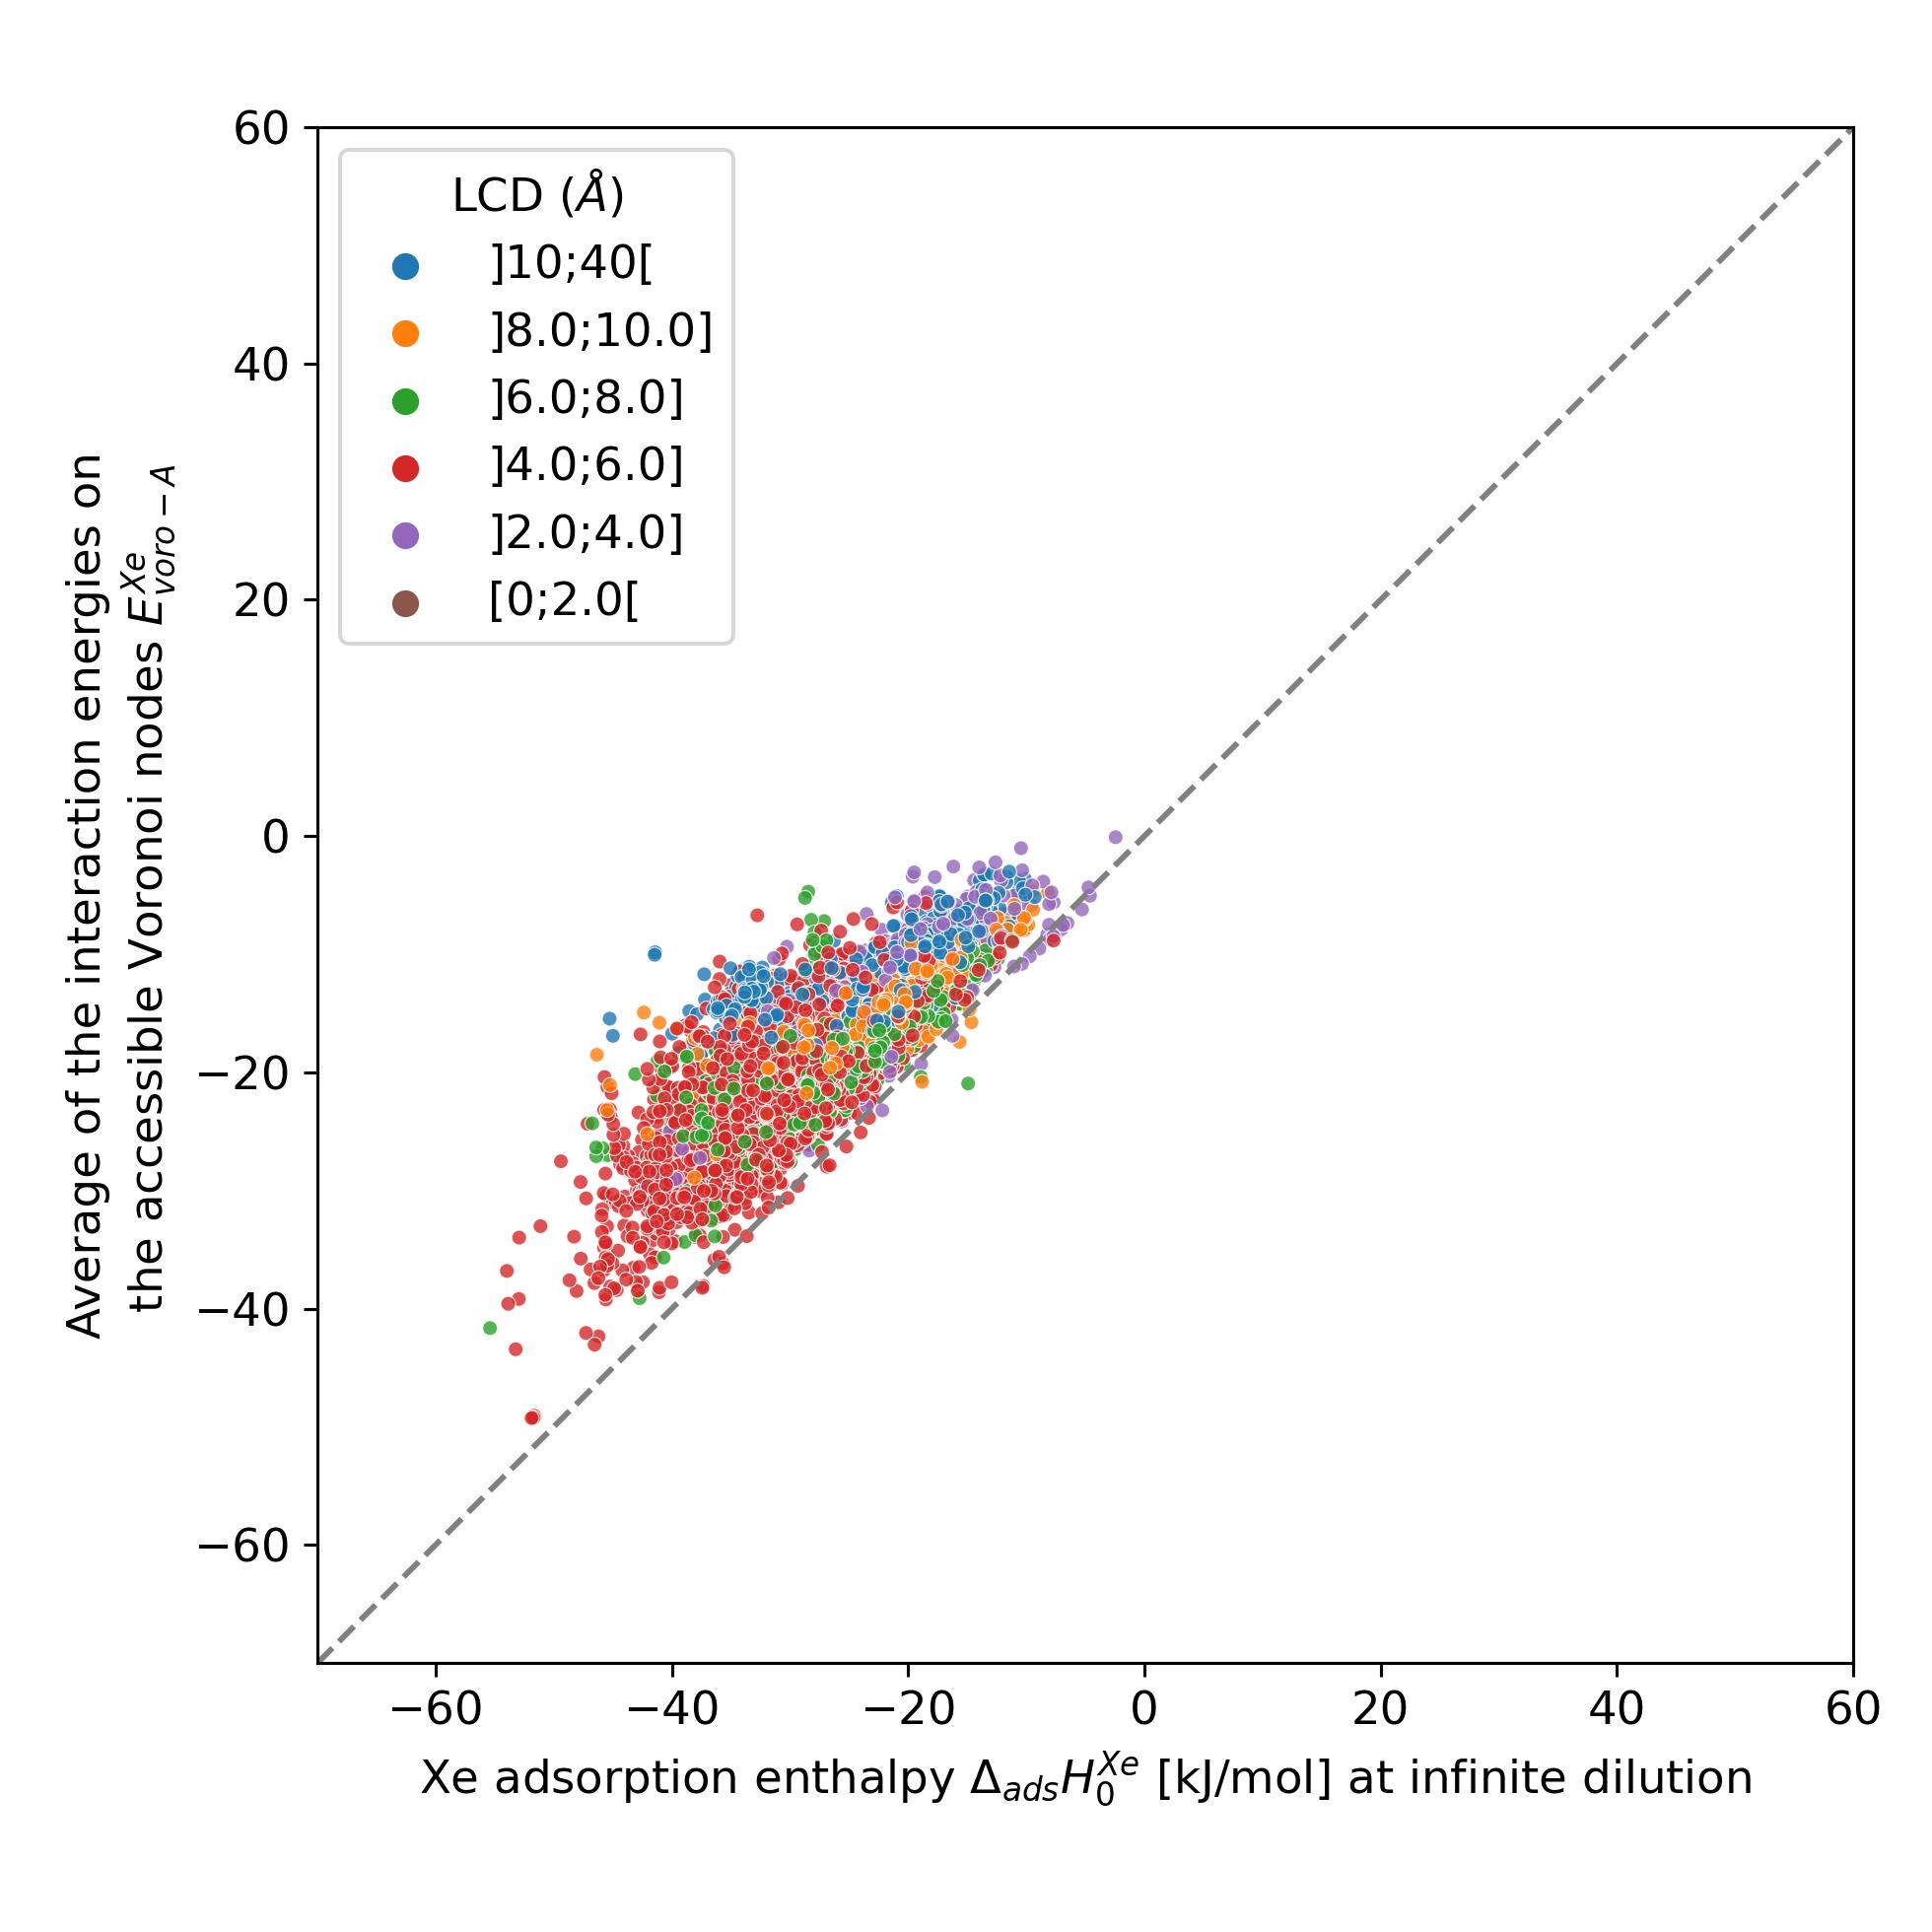
\includegraphics[width=0.32\textwidth]{figures/3-fastsim/H_Xe_0_vs_E_voro_A_overview.jpg}
    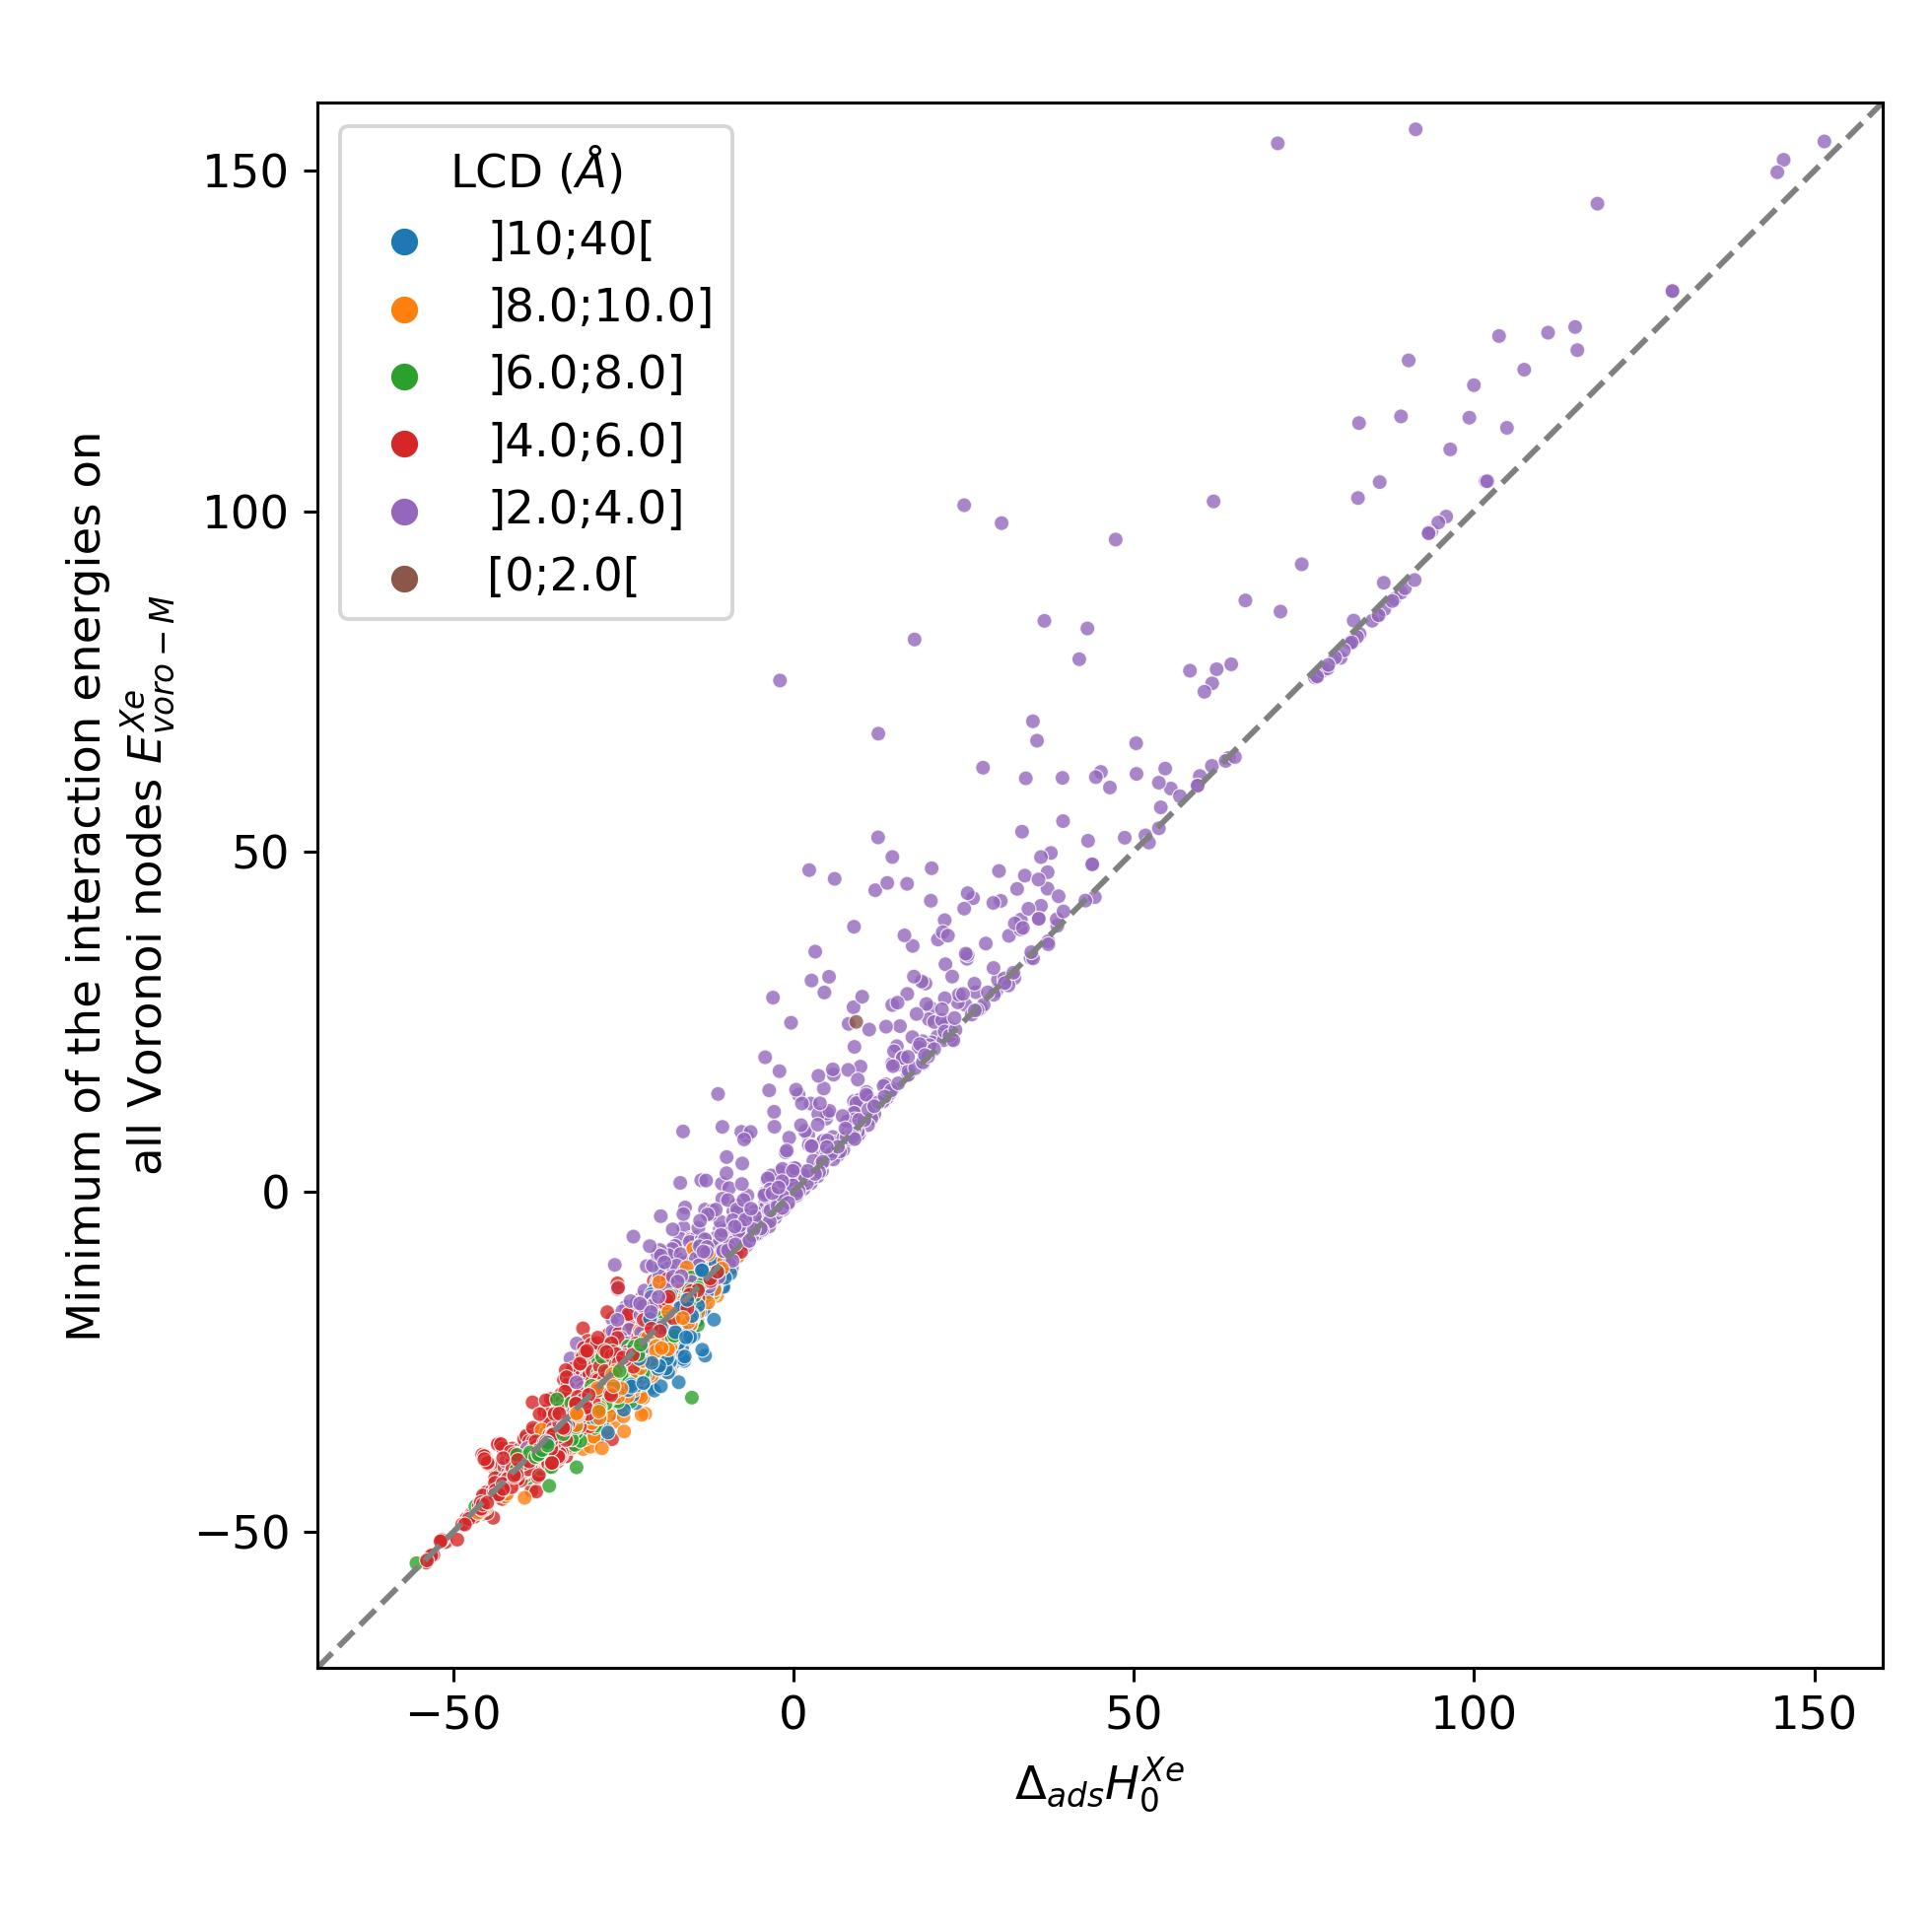
\includegraphics[width=0.32\textwidth]{figures/3-fastsim/H_Xe_0_vs_E_voro_M_overview.jpg}
    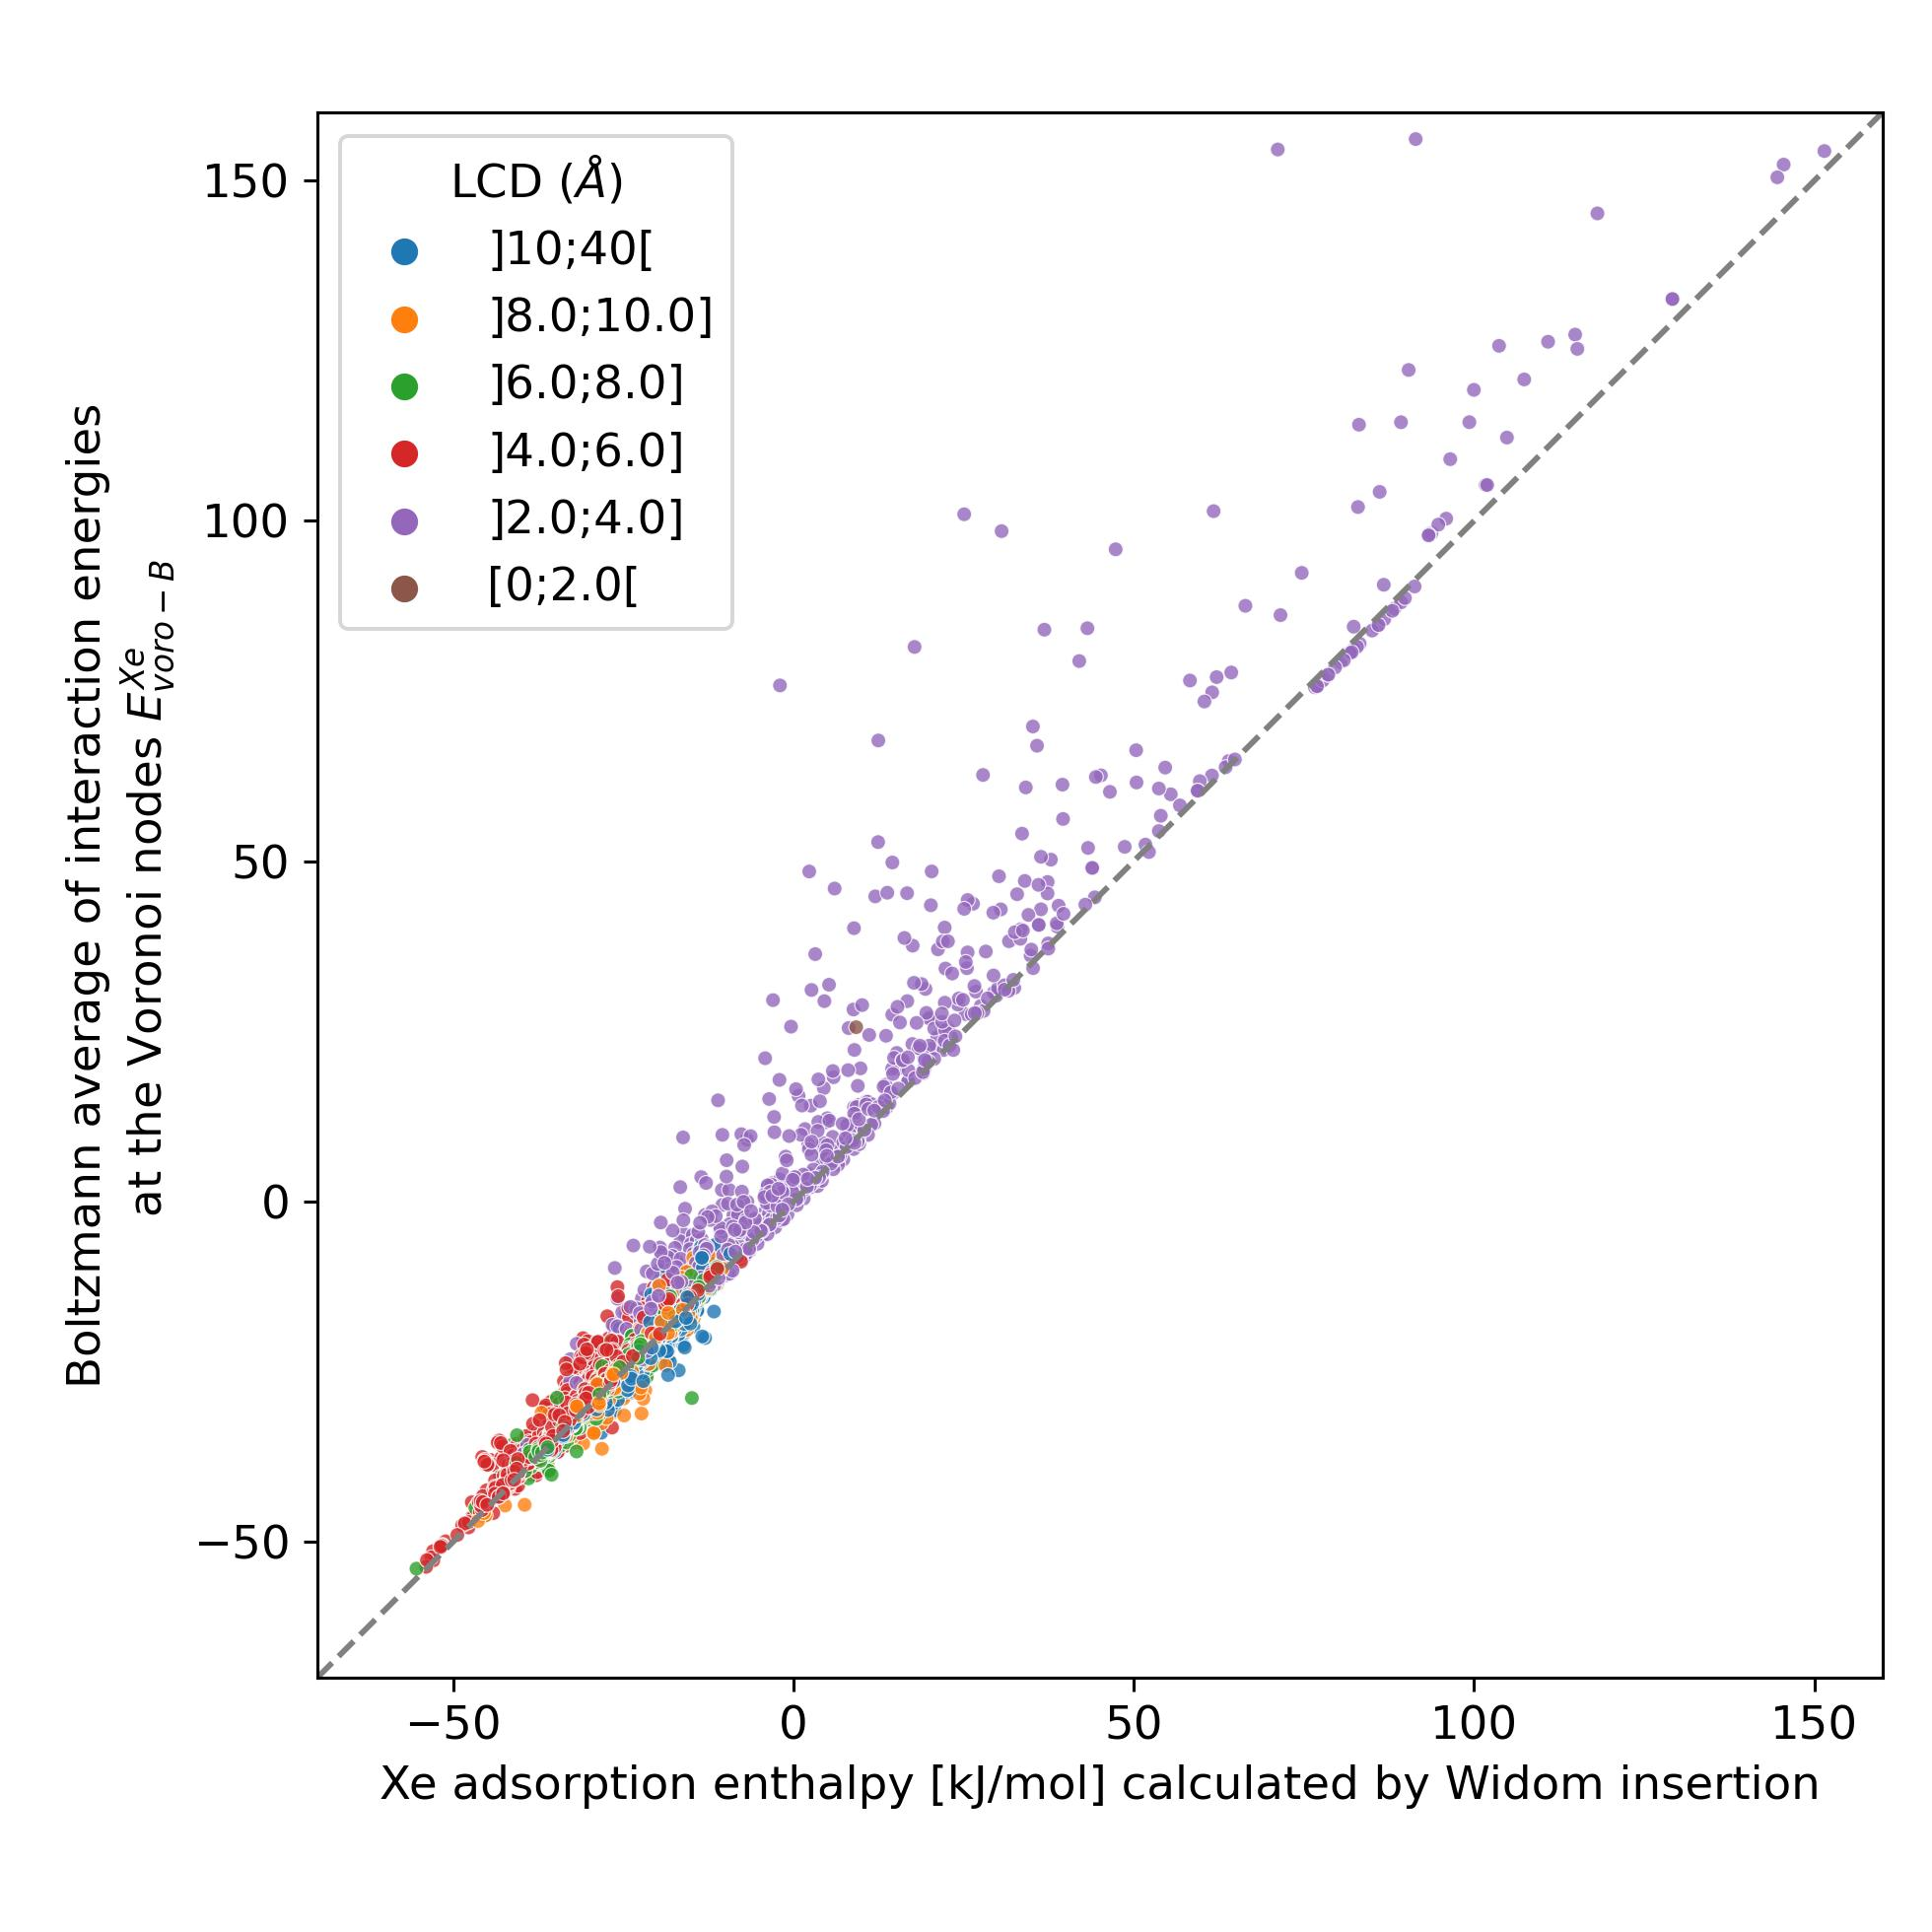
\includegraphics[width=0.32\textwidth]{figures/3-fastsim/H_Xe_0_vs_E_voro_B_overview.jpg}
    \caption{Scatter-plot of the enthalpies calculated by a Voronoi sampling comparedto the enthalpies calculated by a 100k step Widom insertion simulation of xenonin structures of CoRE MOF 2019. The points are labeled according to the largestcavity diameter (LCD) belonging to one of the intervals.}\label{fgr:comp_voro_0}
\end{figure}


\subsubsection{Ambient pressure}

\begin{figure}[ht]
    \centering
      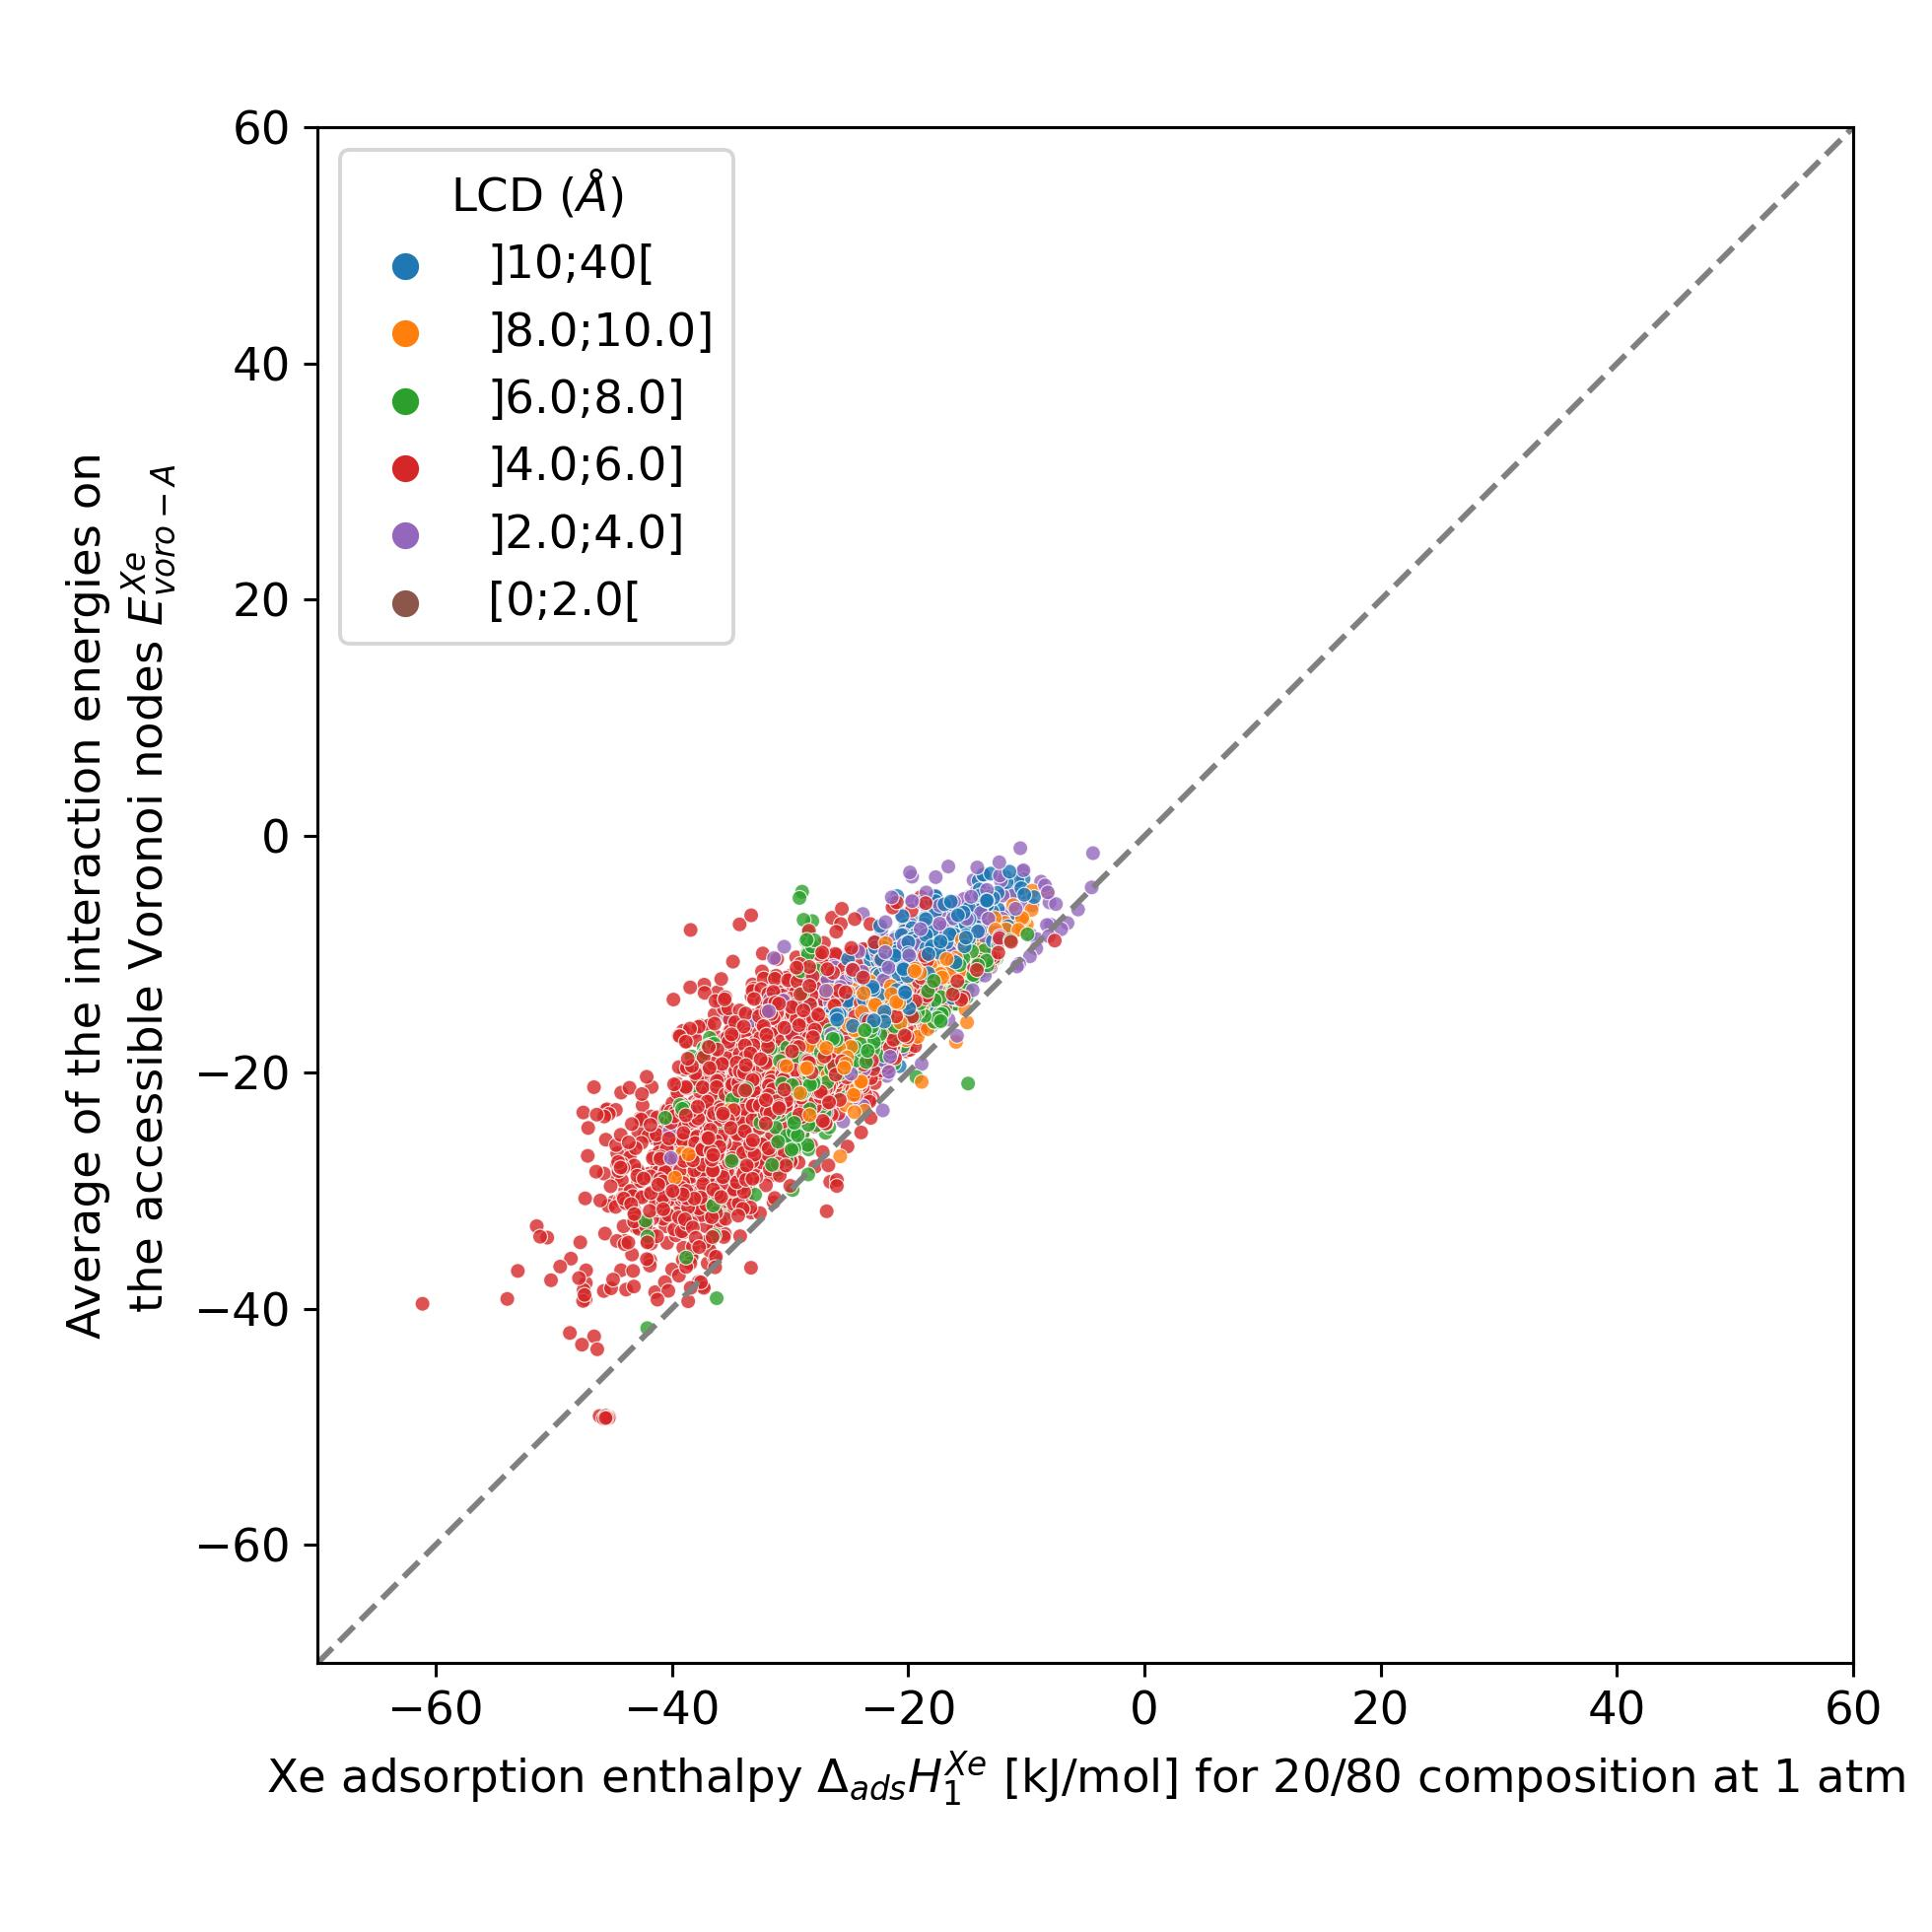
\includegraphics[width=0.32\textwidth]{figures/3-fastsim/H_Xe_2080_vs_E_voro_A_overview.jpg}
      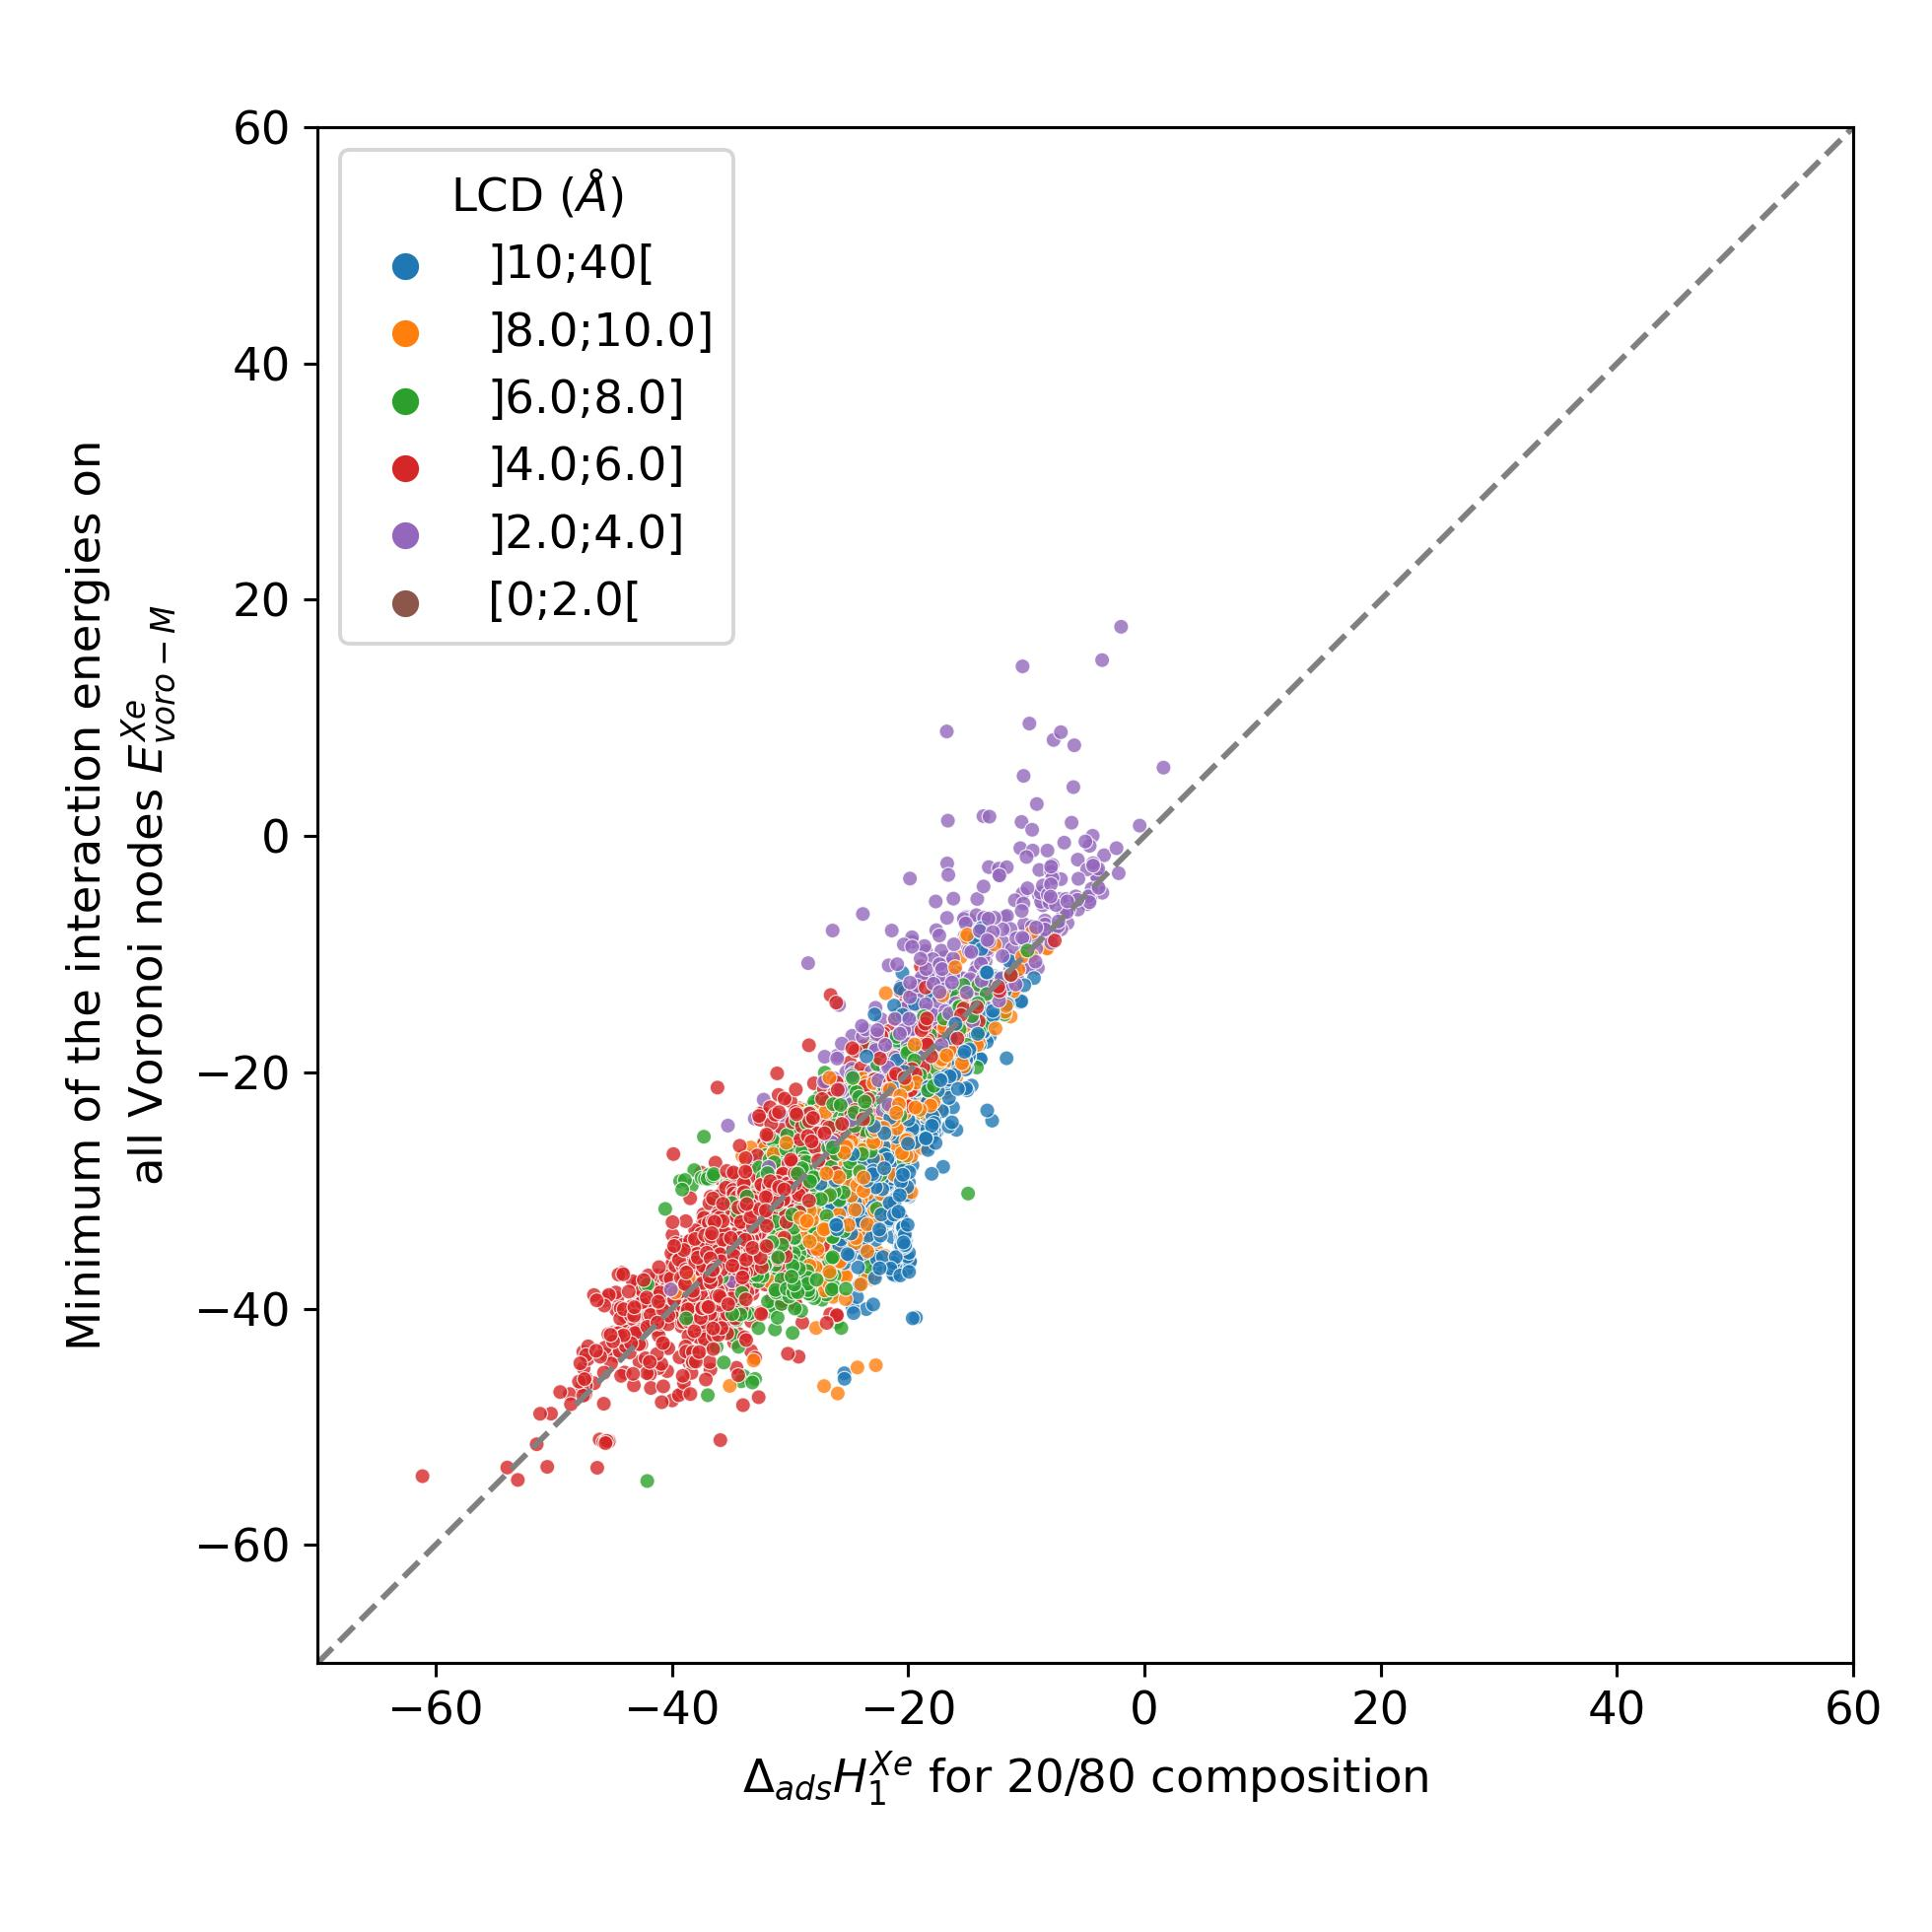
\includegraphics[width=0.32\textwidth]{figures/3-fastsim/H_Xe_2080_vs_E_voro_M_overview.jpg}
      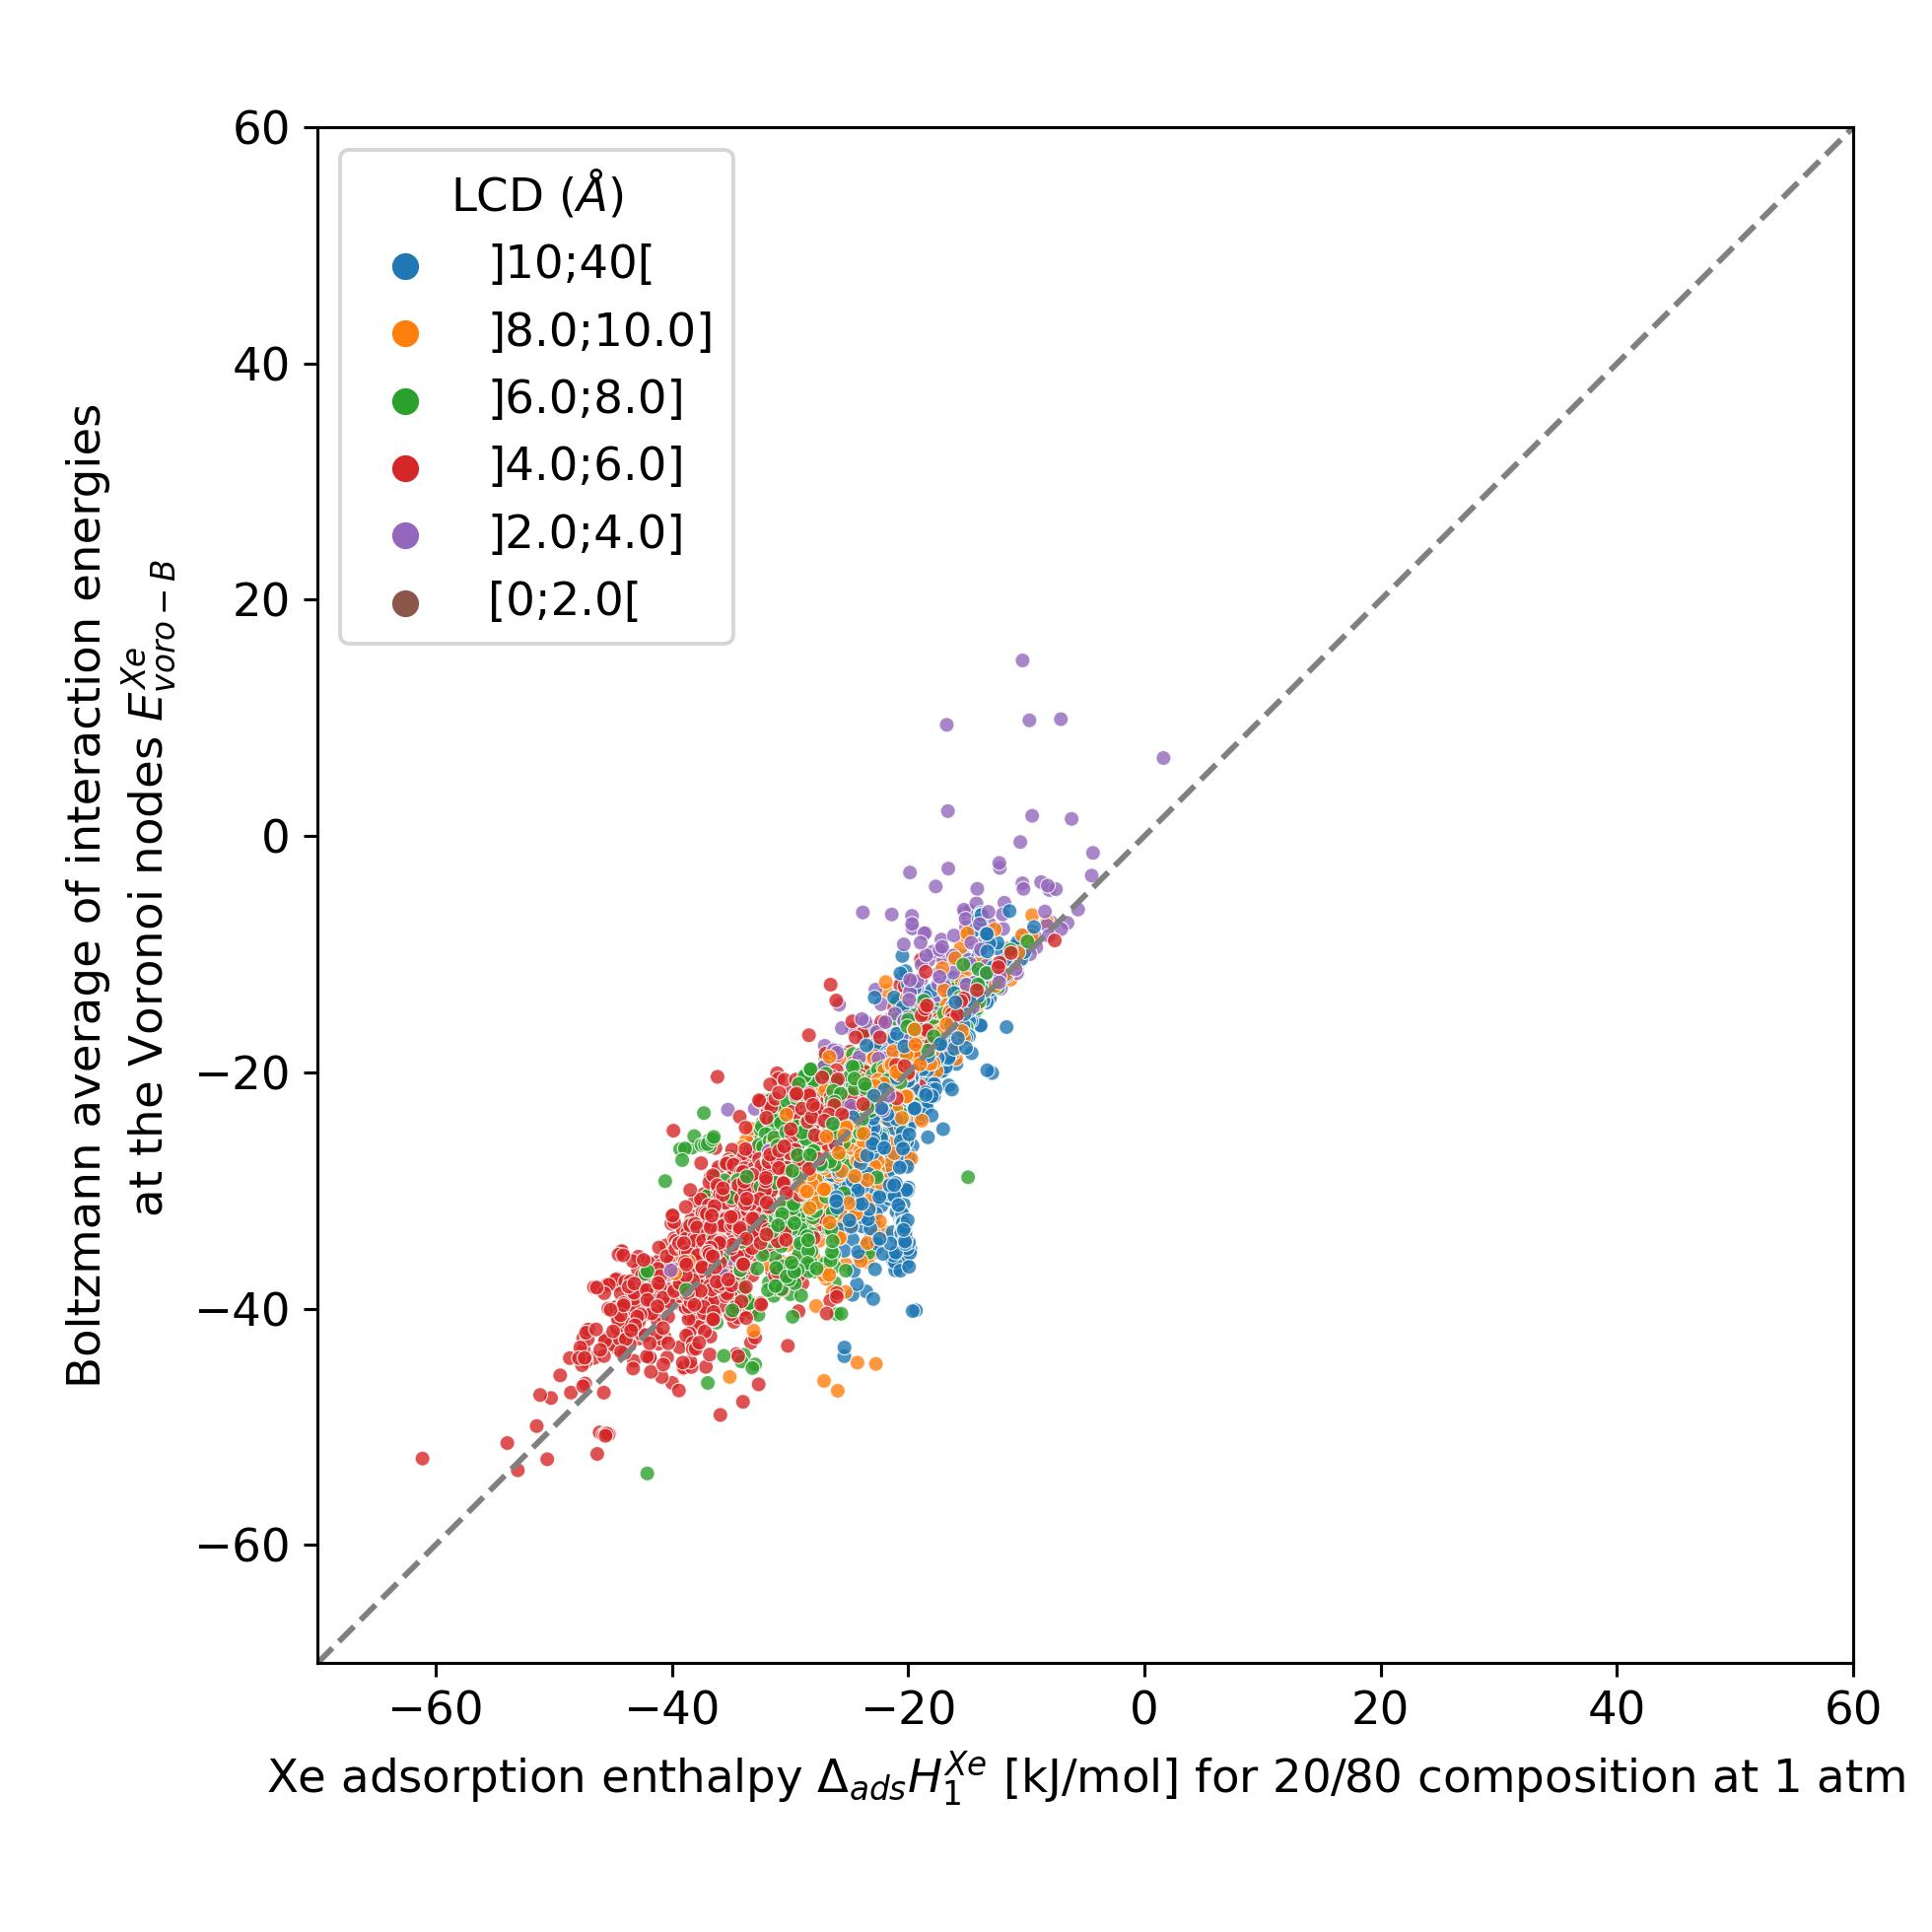
\includegraphics[width=0.32\textwidth]{figures/3-fastsim/H_Xe_2080_vs_E_voro_B_overview.jpg}
      \caption{Scatter-plot of the enthalpies calculated by a Voronoi sampling comparedto the enthalpies calculated by a 100k step Widom insertion simulation of xenonin structures of CoRE MOF 2019. The points are labeled according to the largestcavity diameter (LCD) belonging to one of the intervals.}\label{fgr:comp_voro_2080}
  \end{figure}
  


\subsection{Efficiency of the method}

To check the accuracy of this sampling technique, we compared it to our reference sampling, the Widom insertion with 100,000 cycles. Figure~\ref{fgr:voronoi} compares the enthalpy computed in the Voronoi sampling with the reference adsorption enthalpy (ground truth) --- showing at the same time the largest cavity diameter for each porous framework. The correlation between the values of enthalpy is very good only for a restricted number of structures with enthalpy around \SI{-50}{\kilo\joule\per\mole}. For structures with higher enthalpy, the correlation starts to degrade, and becomes very poor for small-pore structures. For the points in purple, the largest cavity diameter is lower than the kinetic diameter of a xenon, the sampling of the Voronoi nodes is clearly insufficient. In addition, the accuracy loss on the other points (larger pores) can be explained by the fact that the pores are slightly bigger and the center of the pore is not a good approximation of adsorption site position anymore: the adsorption sites are actually closer to the pore surface than to the center of the pore. This conclusion is what prompted us to propose a new sampling scheme based on the molecular surface of the pore space, which we will detail in the next sections.

The root mean square error (RMSE) {and the mean absolute error (MAE) for Voronoi sampling are respectively \SI{6.78}{\kilo\joule\per\mole} and \SI{2.01}{\kilo\joule\per\mole}}, if we consider all structures in our set, which seems too high to be useful for screening purposes. However, the non-porous materials would be screened out \emph{a priori} in any high-throughput workflow, as they would not be of interest. We can only consider the structures with large enough cavities, higher than \SI{3.7}{\angstrom} (a bit lower than \SI{3.96}{\angstrom} Xe kinetic diameter). Thereby, {the RMSE and MAE drop respectively to \SI{2.11}{\kilo\joule\per\mole} and \SI{1.55}{\kilo\joule\per\mole}}, which can be considered acceptable for a quick estimation of the guest--host affinity, but not for accurate adsorption enthalpy calculation.

This is reinforced by the very low computational cost of the method. The Voronoi tessellation done by the Zeo++ software is extremely quick and can output the positions of the Voronoi nodes in \SI{0.28}{\second} (measured as an average over all the structures of the CoRE MOF 2019 database), on a typical workstation (a single Intel Xeon Platinum 8168 core at 2.7~\si{\giga\hertz}). While a simple Python for the energy calculation took around \SI{27}{\second} per structure, we benchmarked that a C++ optimized implementation can perform the Voronoi sampling in around \SI{0.4}{\second}. We only need to remember that this method takes a few hundred milliseconds per structure, while a Widom insertion needs approximately hundreds of seconds per structure. A Voronoi sampling is therefore 2 to 3 orders of magnitude quicker than a full sampling of the pore space.

This preliminary study identified a fast method for adsorption enthalpy calculation that can be widely used in screening procedures, but has limited accuracy for quantitative prediction. It raised important questions on the importance of selecting sampling points within the pore space of materials, and we wanted to develop an intermediate technique that is both fast and accurate for the prediction of adsorption enthalpy. For this purpose, we developed and optimized a new sampling technique that focuses the sampling on the surface of the material, which is expected to make up for the main flaws of the Voronoi sampling.



\section{Rapid Adsorption Enthalpy Surface Sampling (RAESS)}

In this section we describe the development of our surface sampling algorithm, with the goal of being more accurate than Voronoi sampling and faster than Widom insertion. Our initial idea is based on a series of theoretical considerations: (1) the strong adsorption sites are near the surface of the material; (2) by changing the problem from 3D to 2D sampling we can reduce the complexity; and (3) the algorithm can scale with the number of unique atoms in the structure (and not with the size of the unit cell), which is efficient because many porous frameworks have high symmetry. The first consideration ensures that this method will be more accurate than a Voronoi sampling, and the last two made us think that a well-optimized code would be fast. To confirm these hypotheses, we will analyze both the accuracy and the speed of this new algorithm and compare them to existing methods.

\subsubsection{Initial implementation}

We present here our initial implementation of the surface sampling algorithm, and its basic principles. This first implementation is a relatively basic one and already performs well compared to the other methods. In the next sections, we refine it with two additional features that will improve its accuracy and its speed.

This initial implementation speeds up the calculation of adsorption enthalpy in nanoporous materials by sampling interaction energies only near the surface. It is illustrated in Figure~\ref{fgr:principle}. For this purpose, a loop over all unique atoms (as defined by crystalline symmetry) is performed. And for each atom, a sphere around its position is sampled using a uniform distribution around it, these points will be called sampling points and we can change the number of sampling points. The default radius chosen for the sampling spheres is the distance $r\e{min}=2^{1/6}\sigma_{ij}$ to the minimum of the LJ potential between atoms of type $i$ (belonging to the framework) and $j$ (the guest), corresponding to the strongest possible pair interaction (although the neighboring atoms will of course have an influence). After calculating the interaction energy at each of the sampled points, a Boltzmann average of these energies corresponds to a biased adsorption enthalpy, as described by the equation~\ref{eq:enthalpy}.

\begin{figure}[ht]
\centering

  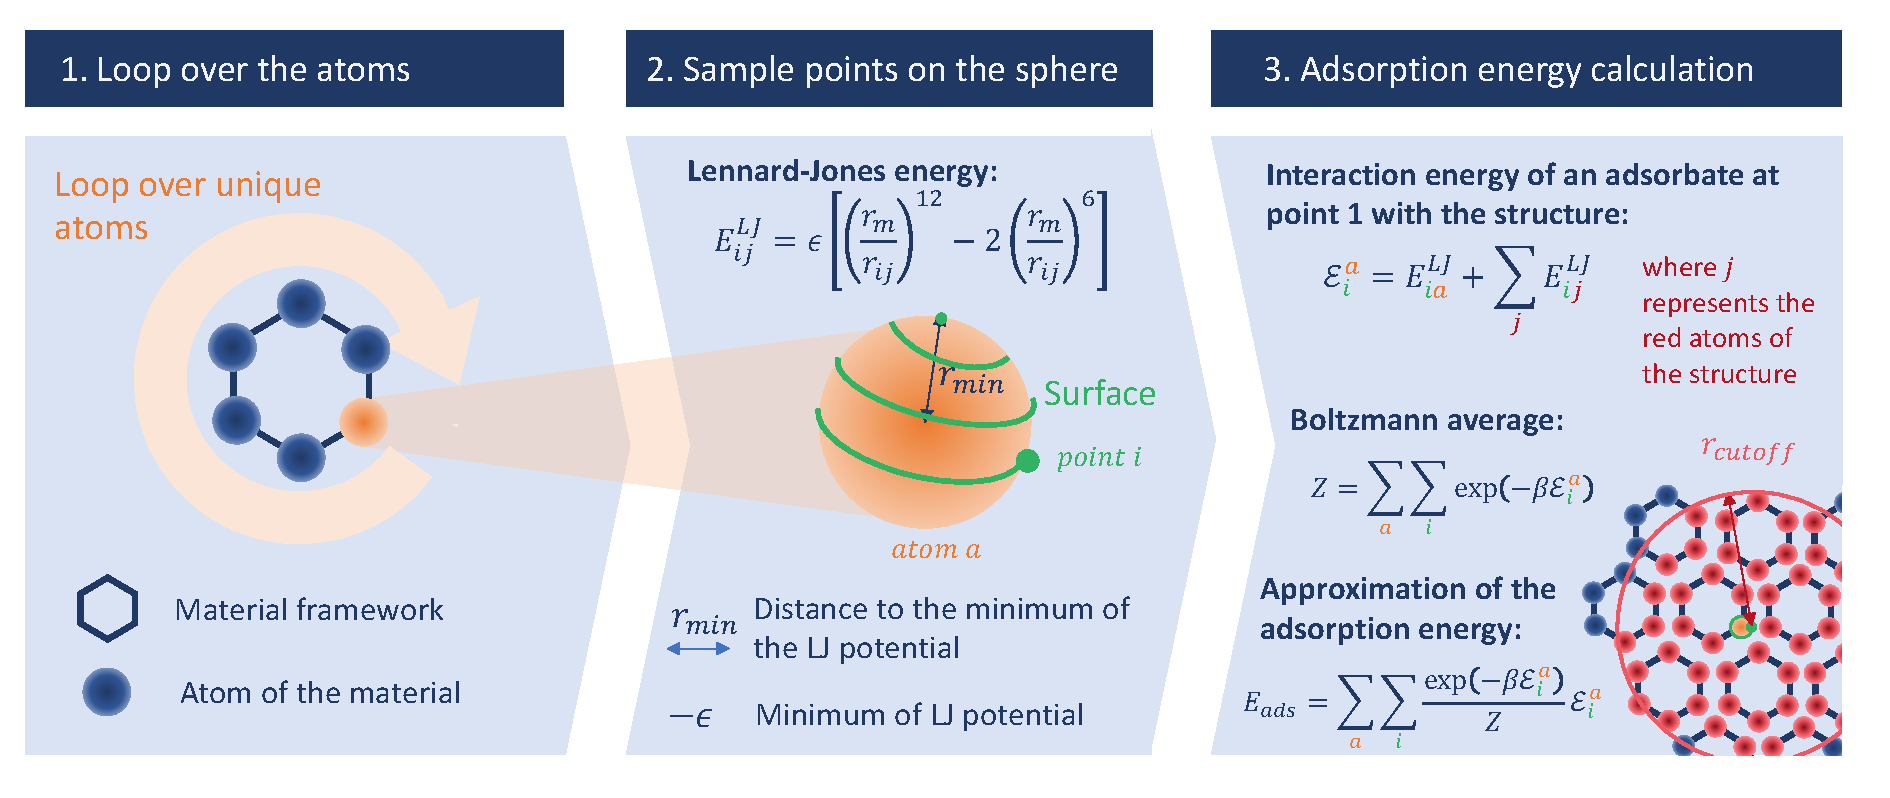
\includegraphics[clip, trim=0.6cm 0.74cm 0.78cm 0.6cm,width=0.95\linewidth]{figures/3-fastsim/Principe_screening.pdf}
  \caption{Schematic description of our surface sampling based on the three main steps of the algorithm: the loop over the unique atoms, the {spiral} sampling around each atom, and the energy averaging. {The adsorbate is represented by the point $i$ and is moved across all the points around the unique atoms of the structure. } }
  \label{fgr:principle}
\end{figure}

In order to validate the accuracy of the approximation made using this sampling, we applied this algorithm with 300,000 sampling points per unique atom. The results are illustrated by the Figures~S1 and S2 and Table~S1 of the supporting information (SI). There is a good numerical agreement with the reference calculations, {the RMSE and MAE are only around \SI{0.90}{\kilo\joule\per\mole} and \SI{0.66}{\kilo\joule\per\mole}} considering all the structures from the database. Moreover, there is no noticeable difference of RMSE when considering the structures with a pore size above \SI{3.7}{\angstrom} (as determined by the largest cavity diameter, or LCD). Unlike Voronoi sampling, this method gives a consistent accuracy across all the structures of the database with a lower error. The fact that the {RMSE} error is below \SI{1}{\kilo\joule\per\mole} is quite promising, and validates our intuition that this new sampling technique can be an intermediate between to the two previous methods (Voronoi and Widom).

\begin{figure}[ht]
\centering
  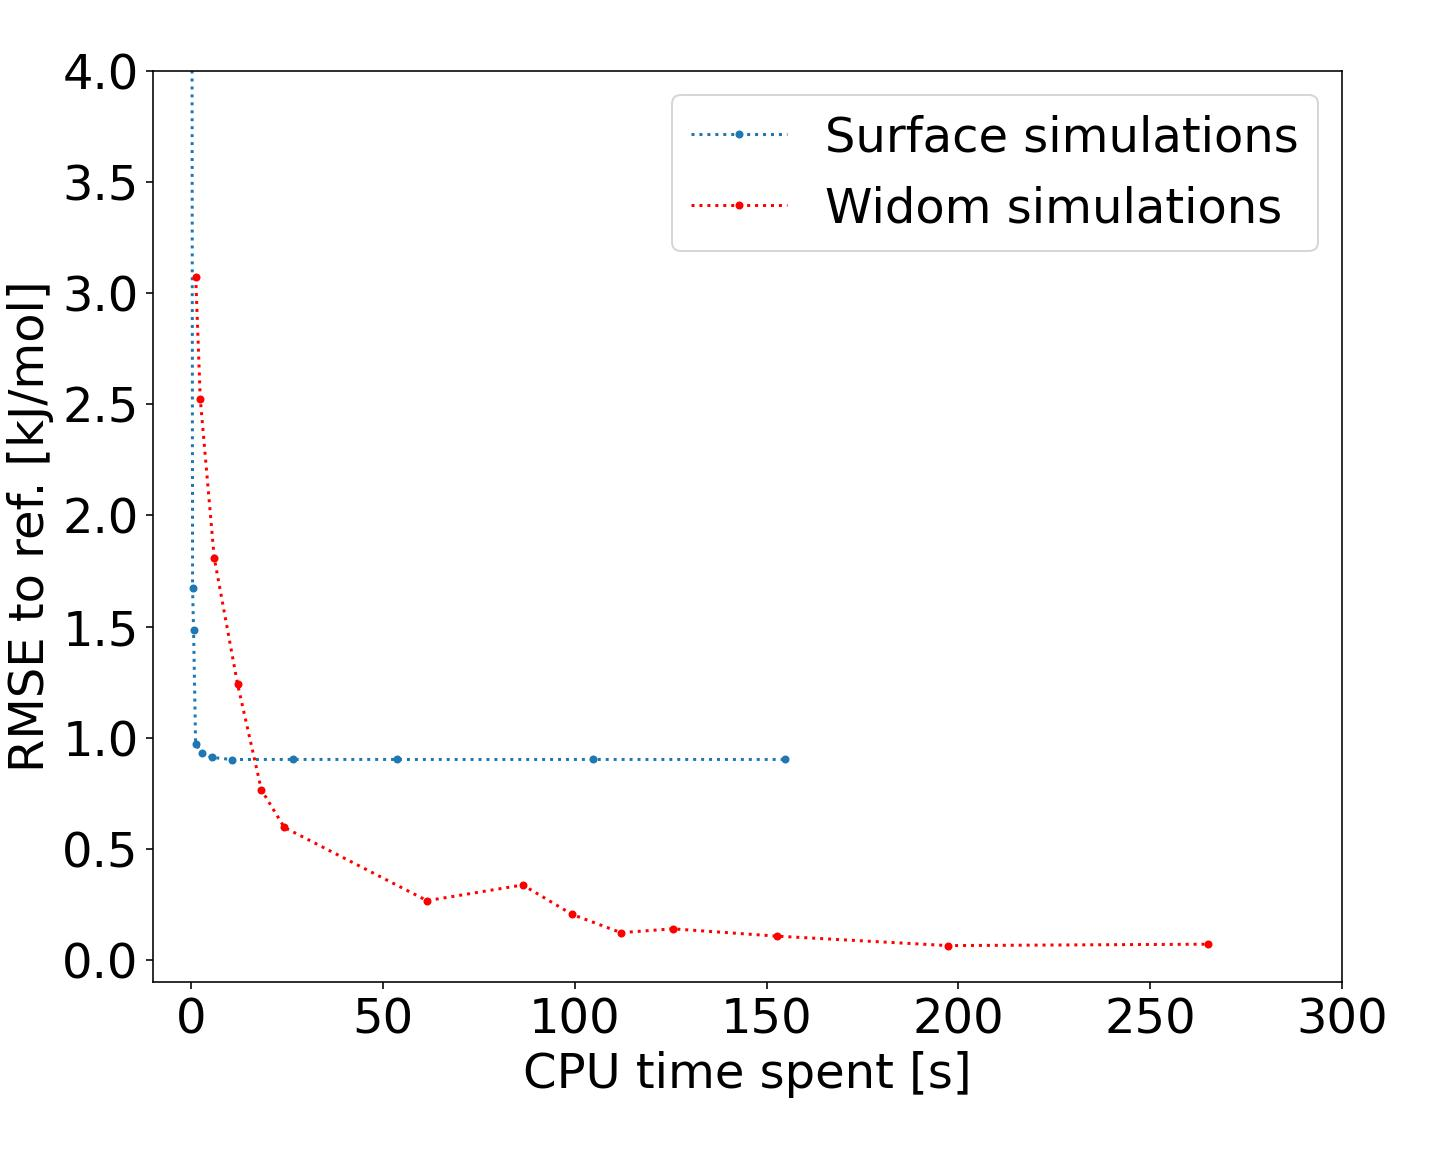
\includegraphics[width=0.7\linewidth]{figures/3-fastsim/time_rmse.jpeg}
  \caption{RMSE convergence of our algorithm (left) compared to a 100k-step Widom insertion simulation (right) for xenon adsorption in {all} structures of the CoRE MOF 2019 database.}\label{fgr:convergence}
\end{figure}

After proving the good accuracy of the method, we are now exploring the computation time required. We see on Figure~\ref{fgr:convergence} that the method reaches an RMSE below \SI{1.0}{\kilo\joule\per\mole} very quickly for an average CPU time of \SI{1.2}{\second} (Table~S1), corresponding to 2,000 sampling points per atom. This is far less than the \SI{150}{\second} (Table~S2) required for a Widom insertion to reach its plateau value, for an RMSE of \SI{0.10}{\kilo\joule\per\mole} with 12,000 cycles. Moreover, the Widom insertion needs around \SI{14}{\second} to reach a similar RMSE of \SI{1.0}{\kilo\joule\per\mole}, which is still slower than the surface sampling. We can conclude that this initial implementation of the surface sampling is faster than a standard Widom insertion, with a good accuracy.

However, this initial implementation of the method is slower than a Voronoi sampling that only needs to sample around 1,600 points on average, instead of 13,000 sampled points on average (if we multiply by the average number of unique atoms). The sampling part would take approximately \SI{0.15}{\second} and the Voronoi nodes generation \SI{0.28}{\second}, so our surface sampling algorithm remains 2 to 3 times slower (implemented in an identical compiled language, in this case C++). In order to improve the accuracy and performance, we have further tweaked the surface sampling method, adjusting the size of the sampling sphere and adopting a fast rejection criterion. The rejection of high-energy points with little contribution to the final enthalpy value can reduce the simulation time, whereas the size of the sampling sphere can improve the accuracy. The initially chosen sphere size is only taking account of the interaction with the closest atom, we therefore chose to set it at the minimum of Lennard-Jones potential. However, the interaction with the neighboring atoms can further stabilize the adsorbate, sampling further from this minimum could in consequence increase the accuracy of our surface sampling method.

\subsubsection{Size of the sampling sphere}

The validity of the initial algorithm is based on the assumption that the adsorption site is at the minimum of the Lennard-Jones potential. It will only perform well if the closest atom contributes to almost all the interaction, but in real frameworks other neighboring atoms contribute to the host/guest interaction as well. We have found that in vast majority of materials, the adsorption sites are located farther apart compared to the LJ potential minimum, in order to maximize the contribution of all atoms --- and because of the dissymmetry of the interaction potential well. In order to see if this could be introduced in our algorithm, we implemented a parameter $\lambda$, and the sampling sphere radius is now defined by $R_{\lambda} = \lambda \sigma$, where $\sigma$ is the distance at which the LJ potential is zero. If $\lambda=2^{1/6}$, we fall back to our initial definition of the sampling sphere, and the adsorbent is at the minimum of the LJ potential of the atom. If $\lambda=1$, the sampling sphere is at the zero of the LJ potential, and by increasing this parameter, we can check if our intuition was right.

\begin{figure}[ht]
\centering
  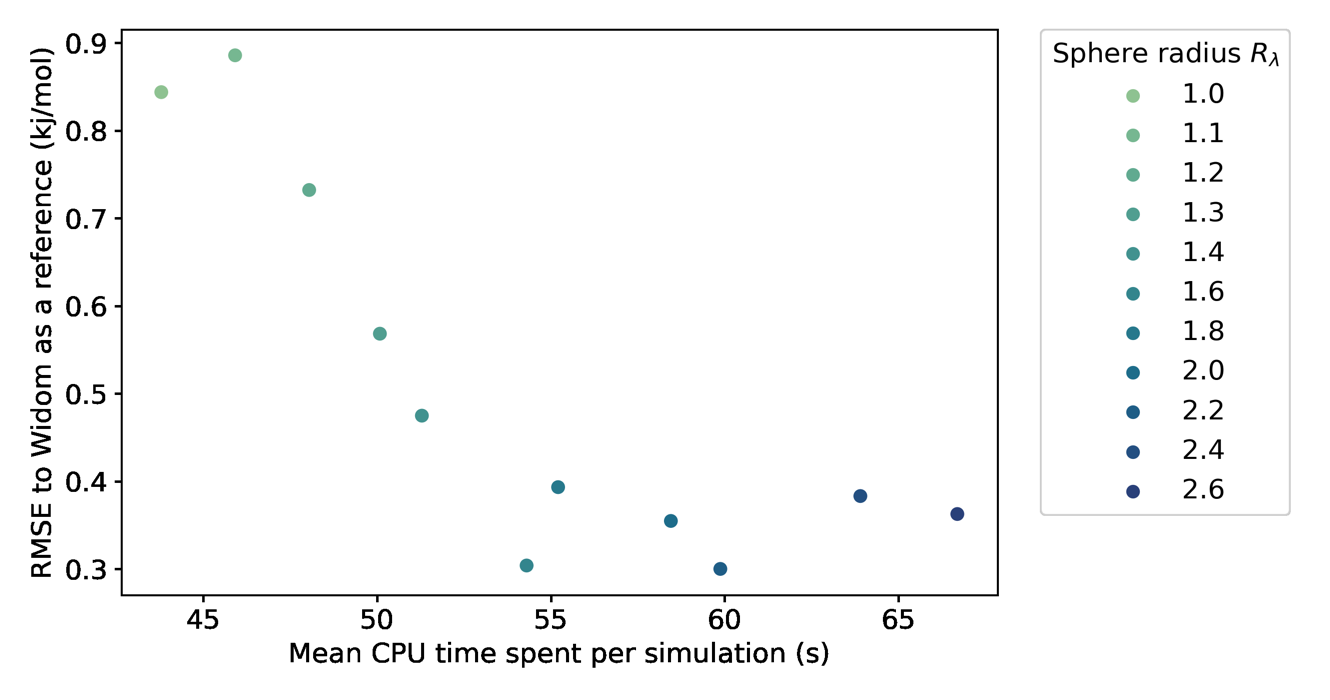
\includegraphics[width=0.7\linewidth]{figures/3-fastsim/sphere_size_optimisation.png}
  \caption{Influence of the sampling sphere radius $R_{\lambda}$ on the average CPU time required for a simulation of 100k sampling points and the RMSE, compared to the reference adsorption enthalpy. The averaging is done only on the structures with a largest cavity diameter (LCD) higher than \SI{3.7}{\angstrom}.}
  \label{fgr:radius}
\end{figure}

Because we have no physical model that would predict the optimal value of the sampling sphere, we followed a statistical approach. We studied the influence of the $\lambda$ parameter on both the accuracy and the computation time, and the results are represented on Figure~\ref{fgr:radius}. The RMSE turns out to be relatively high around \SI{0.90}{\kilo\joule\per\mole} for radius sphere lower than the $r\e{min}$, it then decreases for larger values of radius to reach a plateau around \SI{0.35}{\kilo\joule\per\mole}. We confirm that by increasing the sampling sphere radius we can improve the accuracy of our algorithm, and find that for values of $\lambda$ higher than $1.6$, the accuracy is stabilized. We also find that increasing the sphere radius negatively impacts the computational efficiency, since it increases the number of neighbors considered in the energy calculation.

By choosing an optimal sampling sphere, we can more than halve the error, while increasing the computation time by around 20 percent, when comparing the case $\lambda=1.6$ with $\lambda=1.1$ (close to $r\e{min}$). In most cases, it will be an acceptable trade-off. However, in a case where the computation time is crucial, like in a rapid screening, the optimal choice might not be to increase the sampling sphere at $\lambda=1.6$ but to have it lower at $\lambda=1.4$ or $\lambda=1.2$, and have an RMSE around \SI{0.5}{\kilo\joule\per\mole} --- still quite acceptable. The new scale parameter introduced in this section can therefore be tweaked to serve the users' purpose, whether it is to focus on the accuracy or to optimize the computation speed. {If one wants to use it on a completely different database in very different conditions, then one can either choose a default value that works fine (\emph{e.g.} $\lambda=1.4$) or one can optimize the parameter on a small diverse sample of the unseen data. }

\subsubsection{Rejection condition}

As shown above, our algorithm has better accuracy than Voronoi sampling, but its initial implementation was several times slower, which could be unsuitable for screening applications in high-throughput workflows, where the number of structures to be screened can reach one million or more. To reduce the computational expense, we thought of rejecting the points with little contribution to the final enthalpy, i.e., the largely positive interaction energies that would vanish in the exponential of the  Boltzmann average.

\begin{figure}[ht]
\centering
  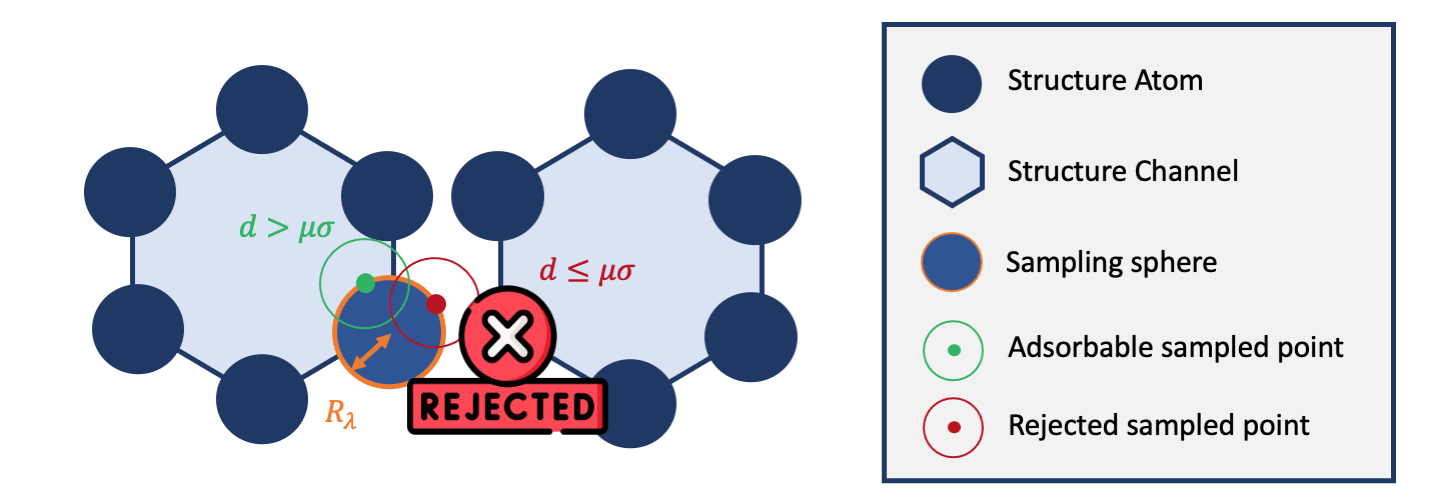
\includegraphics[width=\linewidth]{figures/3-fastsim/rejection_sampling_sphere.png}
  \caption{Simplified representation of the principle of rejection condition and the concept of sampling sphere inside 2D channels of a nanoporous material.}
  \label{fgr:feature}
\end{figure}

Inspired by typical methods for accessible surface calculation, we implemented a hard sphere rejection condition based on the distance to neighbors. If the adsorbate is too close to another atom of the structure, the sampling point is rejected, i.e., its energy is not calculated (or considered to be infinite). We based this distance threshold on the $\sigma_{ij}$ parameter of the Lennard-Jones potential. To determine the optimal threshold, we introduced a factor $\mu$ with real values between 0 and 1, that changes the size of the hard sphere rejection condition. If the guest--host distance is lower than $d_{\mu} = \mu \times \sigma$, then the point is rejected. If $\mu = 0$, then there is no rejection condition. And if $\mu = 1$, we reject all points with a positive energy interaction to at least one atom of the structure. This condition could be a bit strong and points with non negligible contribution would end up rejected. This rejection condition is schematically represented on Figure~\ref{fgr:feature}.

This rejection condition is expected to speed up the calculation, since the energy calculation is avoided for the rejected sampling points. The energy calculation accounts for the largest portion of the CPU time spent in the surface sampling. For the structure \texttt{KAXQIL}\cite{Banerjee_2012}, the Lennard-Jones potential calculation represents up to $90\%$ of the calculation time for 100,000 sampling points per sphere (with the initial algorithm). The higher the factor $\mu$, the more rejections there would be. But, if too many points are rejected, the accuracy would drop. Here again, we used a statistical analysis to determine the optimal value of $\mu$, making our sampling faster without compromising the accuracy of the enthalpy calculation. The results are displayed on Figure~\ref{fgr:rejection}.

\begin{figure}[ht]
\centering
  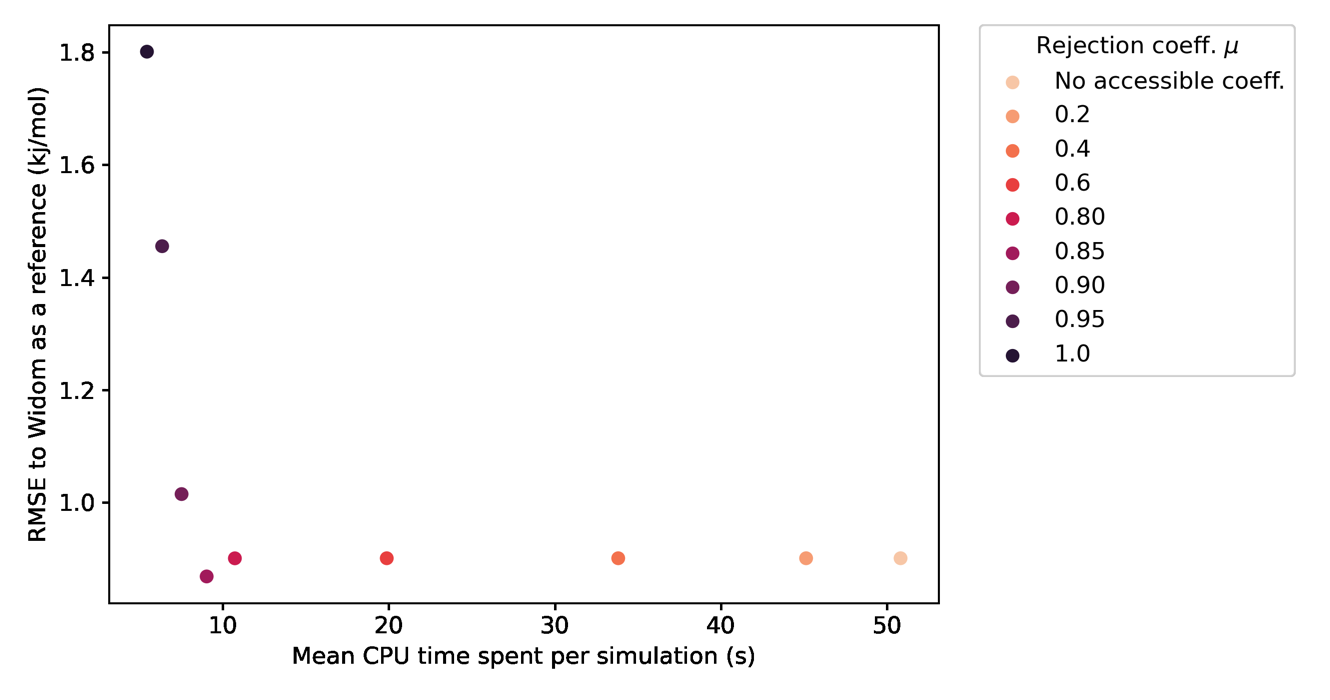
\includegraphics[width=0.7\linewidth]{figures/3-fastsim/rejection_coeff_optimisation.png}
  \caption{Influence of the rejection coefficient $\mu$ on the average CPU time required for a simulation of 100k sampling points and the RMSE compared to the reference adsorption enthalpy. The averaging is done only on the structures with a largest cavity diameter (LCD) superior to \SI{3.7}{\angstrom}. }
  \label{fgr:rejection}
\end{figure}

The values of RMSE and time on Figure~\ref{fgr:rejection} are averaged only on the most interesting structures for xenon adsorption (LCD $\geq$ \SI{3.7}{\angstrom}). For $\mu\leq 0.85$, increasing the value of $\mu$ improves the speed of the calculation without changing the RMSE.\footnote{In fact, what we observe is a deterioration of the accuracy for structures with small pores because the probability of rejection in a confined space is really high and all sampled points end up rejected. But these points are not considered, if we apply the condition on the cavity size (LCD $\geq$ \SI{3.7}{\angstrom}).} For high values of $\mu$, the rejection condition is too strong and we reject points with non-negligible contribution to the overall enthalpy. The RMSE increases as a consequence. If we want to keep the accuracy unchanged, the optimal value is therefore $\mu \simeq 0.85$, because it give the lowest computation time with a similar RMSE. We note that it would be possible, in specific cases, to explore higher values of $\mu$ that trade a bit more accuracy in exchange of further speed gains.

For the simulations considered in Figure~\ref{fgr:rejection}, the use of a rejection condition $\mu = 0.85$ makes the simulation four times faster than the standard algorithm. As we will see in the next section, the combination of optimal values for the $\lambda$ and $\mu$ parameters generates an algorithm with very interesting performance compared to Voronoi sampling or Widom insertion.


\subsection{Final surface sampling algorithm}

\subsubsection{Performance comparison}

For the calculation of adsorption enthalpy, our proposed surface sampling method is a good compromise between the accuracy of Widom insertion (full sampling of the porous space) and the speed of a less accurate method such as Voronoi sampling. The performance of our algorithm, including the two new features (sampling sphere scaling and rejection criterion) is illustrated in Figure~\ref{fgr:sumup}, where we can see the improvement brought by each feature and how it compares to reference simulations. All CPU times are calculated using the smallest possible number of sampling points so that the respective algorithms reach convergence. With the implementation of a rejection condition, we find that surface sampling is even quicker than Voronoi sampling. Moreover, the increase of the size of the sampling sphere makes the surface sampling much more accurate, reaching an RMSE of \SI{0.33}{\kilo\joule\per\mole} {and an MAE of \SI{0.21}{\kilo\joule\per\mole}}. The ideal set of parameters, determined for porous materials from the CoRE MOF 2019 database, is $(\lambda = 1.6, \mu = 0.85)$ in order to combine the lowest error and smallest computational cost. By combining both of these new features to the algorithm, we have a final surface sampling method with an RMSE of \SI{0.33}{\kilo\joule\per\mole} and an average computation time of \SI{0.34}{\second} per structure. According to the data of the Table~S3, it is about 6 times more accurate and {$26$\%} faster than Voronoi sampling, and it is also about 430 times faster than a Widom insertion with 12k cycles.

\begin{figure}[ht]
\centering
  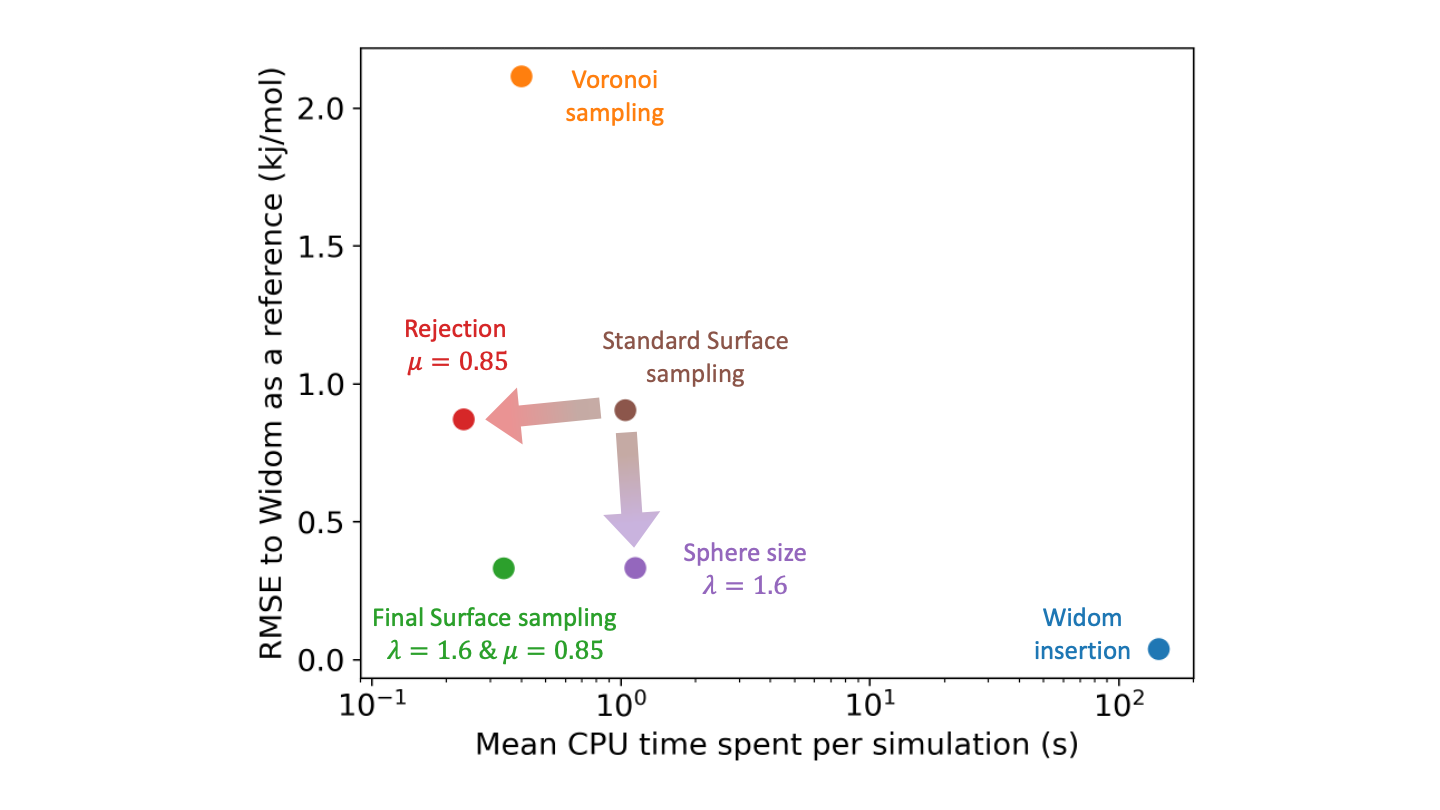
\includegraphics[width=\linewidth]{figures/3-fastsim/methods_comparison.png}
  \caption{Comparison of the RMSE to the reference Widom insertion and the average computation time for different types of enthalpy calculation methods. The surface sampling calculation were all done with 2k sampling points on each sphere and the Widom simulations were done using 12k cycles. These values correspond to the value at the convergence identified using Figure~\ref{fgr:convergence}. }\label{fgr:sumup}
\end{figure}

Finally, we suggest that the values of the parameters optimized in this work might need adjustment when applied to other adsorption systems. The optimal $\mu$ parameter depends on the size of the adsorbent, and it should be tweaked differently when considering another adsorbent. For instance, the set of structures used for the optimization of $\mu$ depends on the size of their cavities, and the \SI{3.7}{\angstrom} threshold chosen here would need to be changed according to the kinetic diameter of the adsorbate. Furthermore, as aforementioned in the section on the rejection condition, it is possible to trade-off a bit of accuracy for faster simulations especially in high-throughput screenings where speed is extremely important. Similarly, in the case of xenon, the cost of increasing the sphere size is around $10$ to {$20$\%}. On very large databases, one could consider that this increase on the required computational time is not worth the accuracy improvement, and one could decide to keep a smaller sampling sphere. If this method is transposed to different molecular systems, its parameters should be tested on the specific database and adsorbate of interest.


\subsubsection{Calculation of Henry constant and surface area}

The main goal of our sampling algorithm is to calculate adsorption enthalpy in the zero-loading limit. But the method can also calculate at the same time the Henry constant and surface area of the materials, without significant additional computational cost. The Henry constant is a key metric for assessing the affinity of an adsorbate to a nanoporous structure. The A/B gas selectivity at low pressure is defined as a ratio of Henry constants of components A and B. This important property can be calculated using Equation~\ref{eq:henry} in a Widom insertion calculation. Instead of using the interaction energies at the Widom inserted points, we can now use the surface sampled points to get an approximate value for the Henry constant.

Using the optimized set of parameters for surface sampling, we assessed the performance of our algorithm on the values of Henry constant by comparing them to ground truth obtained by 100,000 cycles of Widom insertion. Since the Henry constant corresponds to the exponential of an adsorption free energy and we are more interested in the precision on the free energy, we are using a log-scale evaluation metric. For surface sampling, the log-RMSE of $K\e{H}$ is equal to $0.2$, which means that the order of magnitude of the values are well predicted (Table~S4). If we consider the derived free energy $\Delta F_{ads} = -RT \log(\rho_fRT K_H)$, the RMSE is of the order of \SI{1.1}{\kilo\joule\per\mole} reached in about \SI{1}{\second} (Table~S6). Whereas for Widom insertion, this level of error is also reached in a similar amount of time and \SI{0.1}{\kilo\joule\per\mole} of RMSE is reached in about \SI{86}{\second} (Table~S7). For free energy calculation, surface sampling is still 86 times faster to converge. If consider that the main target is the adsorption enthalpy, the Henry constant is calculated with little additional computational cost and with reasonable accuracy: we get two thermodynamic properties of interest for the price of one.

The same goes for the determination of the surface area. We can adapt our algorithm to count the number of points of the sampling spheres that have a negative energy. These represent the points were a guest molecule can favorably interact, therefore when dividing it by the number of sampled points, we obtain a proportion of adsorbable area of the sphere. Summing this over all atoms, we obtain a total surface area. This implementation is summed up in Equation~\ref{eq:sa}:
\begin{equation}
\label{eq:sa}
    \textrm{SA} = \dfrac{1}{V}\sum_{a\in \textrm{cell}} \dfrac{N\e{accessible}(a)}{N\e{total}}4\pi r(a)^2
\end{equation}
where $V$ volume of the cell $a$ atoms of the cell; $N_{accessible}(a)$ accessible points around the atom $a$; $N_{total}$ sampling points; $r(a)$ radius of the sampling sphere around the atom $a$.
When we set $\lambda=1$, we are sampling spheres that have a radius $\sigma$ and it is equivalent as considering hard spheres all defined by $\sigma$ (convention used by RASPA2 to calculate surface areas). If we compare simulation with $\lambda=1$, we obtain surface areas that are very close to the one obtained by RASPA2 (see Figure~S11 in SI). However, when we consider $\lambda=1.6$, we lose the perfect accordance previously obtained and the points weakly correlated in log-scale (see Figure~S10 in SI). The difference can be explained by the fact that the sphere size is larger, but the proportion of adsorbable points also changes. The relationship between these two adsorption surface areas is no trivial at all. Since the calculation of surface areas is quite cheap, this implementation would not be very useful, except for having a rough idea of the surface area.


\subsection{Conclusions and perspectives}

In the present article, we described a novel algorithm for the high-speed calculation of adsorption enthalpy in nanoporous materials, that takes a unique approach to reduce the sampling necessary. This new algorithm is based on the core principle of dimensional reduction, from a volume problem to a surface one. The algorithm is proven to be significantly faster than the reference Widom insertion (random sampling of porous space). Moreover, the error associated is found to be of the order of \SI{0.4}{\kilo\joule\per\mole}, tested throughout the entire CoRE MOF 2019 database, for xenon adsorption. Even when comparing to existing very fast sampling techniques such as the Voronoi sampling, this surface sampling technique requires similar CPU time, combined with a better accuracy. 

Based on these results, this algorithm has important potential for applications in the current computational analysis workflows of material databases, such as high-throughput screening studies. For instance, this algorithm can be used to get a fast approximation of the low-loading adsorption enthalpy of a molecule inside nanoporous materials. This cheap evaluation of the enthalpy can be used to screen out the structures with little affinity with the targeted adsorbate molecule. It can also be used as a thermodynamic descriptor for selectivity prediction in a machine learning model, as done by Simon et al.\cite{Simon_2015} The computational speed-up brought by this novel methodology can also enable the screening of materials databases at larger scale in the future.

We note, moreover, that the speed of our method resides in the sampling technique itself, rather than in the actual energy calculation. While we have benchmarked it in this work for a simple Lennard-Jones interaction potential, this sampling technique could equally be used to speed up samplings of space based on more expensive modeling strategies, including polarizable force fields or density functional theory (DFT) calculations. In the literature, the need for cheap \emph{ab initio} grade thermodynamic properties is usually fulfilled by using an importance sampling method based on a classical force field.\cite{Vandenbrande2018} In our method, the description of surface sampling is independent of any force field, and the sampling spheres can be defined according to kinetic radius, van der Waals radius or any other physically relevant distance. {Consequently, given a definition of atomic radii, it is possible to define a surface on which to carry out other types of simulation such as neural network potential, DFT or any other force fields. Although the accuracy or relevance of such a sampling remains an open question, the approach will undeniably speed up the simulations.} This could even be applied to calculate adsorption enthalpies while considering intrinsic structure flexibility,\cite{Witman_2017} a task whose main drawback is the high computation time required. Since surface sampling is hundred of time faster than standard methodologies, we could use hundreds of snapshots in a flexibility-aware calculation.

Finally, although the algorithm in its present form can already be applied in a wide range of applications, additional development work could allow us to generalize it to polyatomic adsorbates. For instance, we would need to {work on a definition of the molecular radius for nonspherical adsorbates as well as working} all the orientation conformation of the adsorbent. {We could imagine to make the distance to the surface depend on the orientation of the adsorbate or sample a band volume on the surface. Although the best implementation of the surface sampling for polyatomic adsorbates remains an open question, in theory it should be possible to apply it to more complex adsorbates than the spherical noble gas. } This would add more complexity to the algorithm but would not change the fundamental speedup due to surface sampling, since these orientation moves are also performed in other standard methodologies. To improve even more the accuracy, we could test hybrid samplings with multiple sampling spheres, or a combination of Voronoi nodes and sampling spheres. Another idea could be to have fractions of sphere that are oriented toward the center of pore given by the Voronoi node. In theory, having a wider variety of sampling points can only improve the sampling. There are therefore multiple possible sampling techniques that could be built around the method introduced herein. {The code is made freely available on the group's GitHub, where further development will be released.}


\section{Grid Adsorption Energies Descriptors (GrAED)}

Inspired by our recent work on a faster way of calculating the low-pressure adsorption enthalpy and Henry's constant,\cite{Ren_2023} we designed an approach based on symmetry-respecting grids. These were generated using the Gemmi project's C++ library,\cite{Wojdyr_2022} using an algorithm implemented with the following steps. First, we loop over the framework atoms and the grid points around a sphere of radius $0.8\times\sigma_{g-h}$, where $\sigma_{g-h}$ is the distance at which the LJ potential energy between the guest atom $g$ and the host atom is zero. The LJ potential energy between the guest molecule and the closes host atom is calculated and only the grid points with an energy lower than a predefined threshold (here set to \SI{100}{\kilo\joule\per\mole}) are considered ``unvisited'' and will be recalculated in the following loop, the others are considered blocked by the framework and will be considered already ``visited''. This first loop over the framework atoms aims at filtering out the grid points that are blocked by the framework, and we will refer to this preliminary filtering step as ``blocking'' in the Table~\ref{tab:grid}. Then, a second loop over the ``unvisited'' grid points is performed --- at each increment, if the point is ``unvisited'' we calculate the interaction energy between the guest and all the host atoms within the cutoff, then the symmetric images of this point are filled with the same energy value and are considered ``visited'' by the algorithm. This symmetry-aware grid exploration allows the algorithm to divide the time required by the average number symmetry images --- this module will be referred to as ``symmetry'' in the Table~\ref{tab:grid}. By combining both the ``blocking'' of the high energy grid points and the ``symmetry'' based calculation of the interaction energies, we built a ``fast'' version of the grid calculation algorithm that can compete with our previously developed rapid surface sampling method (RAESS).

To highlight the improvement in performance in this procedure: the average void fraction for a \SI{1.2}{\angstrom} probe radius is equal to $0.16$ and the average number of symmetric images is equal to $5.8$ on the CoRE MOF 2019 database (most MOFs present symmetry operations). On average, the ``blocking'' procedure means that only {$\sim$16\%} of the grid points really need to be calculated. The ``symmetry'' procedure means only {$\sim$17\%} of points need to be considered, and the combination of both reduces the number of useful points to only {2.7\%} of the grid. This leads to a significant reduction in the CPU time of the calculation, as shown in Table~\ref{tab:grid}.

\setlength{\extrarowheight}{0.1cm}
\begin{table}[ht]
    \begin{tabular}{|l|r|r|}
        \hline
        Energy sampling  &  Average CPU & RMSE on adsorption  \\
        method &  time (s)  &  enthalpy (\si{\kilo\joule\per\mole}) \\[0.5mm]
        \hline
        Grid -- naive -- \SI{0.1}{\angstrom} &  71.3 & 0.025  \\[0.5mm]
        Grid -- blocking -- \SI{0.1}{\angstrom} &  18.8 & 0.026  \\
        Grid -- symmetry -- \SI{0.1}{\angstrom} &  16.8 & 0.024  \\
        Grid -- fast -- \SI{0.1}{\angstrom} &  4.8 & 0.023  \\
        Grid -- fast -- \SI{0.3}{\angstrom} &  0.16 & 0.22  \\
        RAESS\cite{Ren_2023}  &  0.34 & 0.34  \\
        Widom\cite{Widom1963} (12k cycles) &  150 & 0.01  \\
        \hline
    \end{tabular}
    \caption{Performance comparison of the new grid method to other standard techniques used to calculate the adsorption enthalpies. The RMSE is calculated by comparing to the values given by a 100k-steps Widom insertion considered as the ground truth. The associated calculations are performed on the CoRE MOF 2019 database with a single Intel Xeon Platinum 8168 core at 2.7~GHz.}\label{tab:grid}
\end{table}

From the energy values of this grid, we can now calculate many useful descriptors that are used in out final model. A fully detailed description of these descriptors as well as their labeling names are given in the Table~S2 of the SI.

\subsection{Energy-based descriptors}




\todo{transition into ML models}

\OnlyInSubfile{\printglobalbibliography}

\end{document}